\documentclass[]{book}
\usepackage{lmodern}
\usepackage{amssymb,amsmath}
\usepackage{ifxetex,ifluatex}
\usepackage{fixltx2e} % provides \textsubscript
\ifnum 0\ifxetex 1\fi\ifluatex 1\fi=0 % if pdftex
  \usepackage[T1]{fontenc}
  \usepackage[utf8]{inputenc}
\else % if luatex or xelatex
  \ifxetex
    \usepackage{mathspec}
  \else
    \usepackage{fontspec}
  \fi
  \defaultfontfeatures{Ligatures=TeX,Scale=MatchLowercase}
\fi
% use upquote if available, for straight quotes in verbatim environments
\IfFileExists{upquote.sty}{\usepackage{upquote}}{}
% use microtype if available
\IfFileExists{microtype.sty}{%
\usepackage{microtype}
\UseMicrotypeSet[protrusion]{basicmath} % disable protrusion for tt fonts
}{}
\usepackage[margin=1in]{geometry}
\usepackage{hyperref}
\hypersetup{unicode=true,
            pdftitle={Data Visualization with R},
            pdfauthor={Claudia A Engel},
            pdfborder={0 0 0},
            breaklinks=true}
\urlstyle{same}  % don't use monospace font for urls
\usepackage{natbib}
\bibliographystyle{apalike}
\usepackage{color}
\usepackage{fancyvrb}
\newcommand{\VerbBar}{|}
\newcommand{\VERB}{\Verb[commandchars=\\\{\}]}
\DefineVerbatimEnvironment{Highlighting}{Verbatim}{commandchars=\\\{\}}
% Add ',fontsize=\small' for more characters per line
\usepackage{framed}
\definecolor{shadecolor}{RGB}{248,248,248}
\newenvironment{Shaded}{\begin{snugshade}}{\end{snugshade}}
\newcommand{\KeywordTok}[1]{\textcolor[rgb]{0.13,0.29,0.53}{\textbf{#1}}}
\newcommand{\DataTypeTok}[1]{\textcolor[rgb]{0.13,0.29,0.53}{#1}}
\newcommand{\DecValTok}[1]{\textcolor[rgb]{0.00,0.00,0.81}{#1}}
\newcommand{\BaseNTok}[1]{\textcolor[rgb]{0.00,0.00,0.81}{#1}}
\newcommand{\FloatTok}[1]{\textcolor[rgb]{0.00,0.00,0.81}{#1}}
\newcommand{\ConstantTok}[1]{\textcolor[rgb]{0.00,0.00,0.00}{#1}}
\newcommand{\CharTok}[1]{\textcolor[rgb]{0.31,0.60,0.02}{#1}}
\newcommand{\SpecialCharTok}[1]{\textcolor[rgb]{0.00,0.00,0.00}{#1}}
\newcommand{\StringTok}[1]{\textcolor[rgb]{0.31,0.60,0.02}{#1}}
\newcommand{\VerbatimStringTok}[1]{\textcolor[rgb]{0.31,0.60,0.02}{#1}}
\newcommand{\SpecialStringTok}[1]{\textcolor[rgb]{0.31,0.60,0.02}{#1}}
\newcommand{\ImportTok}[1]{#1}
\newcommand{\CommentTok}[1]{\textcolor[rgb]{0.56,0.35,0.01}{\textit{#1}}}
\newcommand{\DocumentationTok}[1]{\textcolor[rgb]{0.56,0.35,0.01}{\textbf{\textit{#1}}}}
\newcommand{\AnnotationTok}[1]{\textcolor[rgb]{0.56,0.35,0.01}{\textbf{\textit{#1}}}}
\newcommand{\CommentVarTok}[1]{\textcolor[rgb]{0.56,0.35,0.01}{\textbf{\textit{#1}}}}
\newcommand{\OtherTok}[1]{\textcolor[rgb]{0.56,0.35,0.01}{#1}}
\newcommand{\FunctionTok}[1]{\textcolor[rgb]{0.00,0.00,0.00}{#1}}
\newcommand{\VariableTok}[1]{\textcolor[rgb]{0.00,0.00,0.00}{#1}}
\newcommand{\ControlFlowTok}[1]{\textcolor[rgb]{0.13,0.29,0.53}{\textbf{#1}}}
\newcommand{\OperatorTok}[1]{\textcolor[rgb]{0.81,0.36,0.00}{\textbf{#1}}}
\newcommand{\BuiltInTok}[1]{#1}
\newcommand{\ExtensionTok}[1]{#1}
\newcommand{\PreprocessorTok}[1]{\textcolor[rgb]{0.56,0.35,0.01}{\textit{#1}}}
\newcommand{\AttributeTok}[1]{\textcolor[rgb]{0.77,0.63,0.00}{#1}}
\newcommand{\RegionMarkerTok}[1]{#1}
\newcommand{\InformationTok}[1]{\textcolor[rgb]{0.56,0.35,0.01}{\textbf{\textit{#1}}}}
\newcommand{\WarningTok}[1]{\textcolor[rgb]{0.56,0.35,0.01}{\textbf{\textit{#1}}}}
\newcommand{\AlertTok}[1]{\textcolor[rgb]{0.94,0.16,0.16}{#1}}
\newcommand{\ErrorTok}[1]{\textcolor[rgb]{0.64,0.00,0.00}{\textbf{#1}}}
\newcommand{\NormalTok}[1]{#1}
\usepackage{longtable,booktabs}
\usepackage{graphicx,grffile}
\makeatletter
\def\maxwidth{\ifdim\Gin@nat@width>\linewidth\linewidth\else\Gin@nat@width\fi}
\def\maxheight{\ifdim\Gin@nat@height>\textheight\textheight\else\Gin@nat@height\fi}
\makeatother
% Scale images if necessary, so that they will not overflow the page
% margins by default, and it is still possible to overwrite the defaults
% using explicit options in \includegraphics[width, height, ...]{}
\setkeys{Gin}{width=\maxwidth,height=\maxheight,keepaspectratio}
\IfFileExists{parskip.sty}{%
\usepackage{parskip}
}{% else
\setlength{\parindent}{0pt}
\setlength{\parskip}{6pt plus 2pt minus 1pt}
}
\setlength{\emergencystretch}{3em}  % prevent overfull lines
\providecommand{\tightlist}{%
  \setlength{\itemsep}{0pt}\setlength{\parskip}{0pt}}
\setcounter{secnumdepth}{5}
% Redefines (sub)paragraphs to behave more like sections
\ifx\paragraph\undefined\else
\let\oldparagraph\paragraph
\renewcommand{\paragraph}[1]{\oldparagraph{#1}\mbox{}}
\fi
\ifx\subparagraph\undefined\else
\let\oldsubparagraph\subparagraph
\renewcommand{\subparagraph}[1]{\oldsubparagraph{#1}\mbox{}}
\fi

%%% Use protect on footnotes to avoid problems with footnotes in titles
\let\rmarkdownfootnote\footnote%
\def\footnote{\protect\rmarkdownfootnote}

%%% Change title format to be more compact
\usepackage{titling}

% Create subtitle command for use in maketitle
\newcommand{\subtitle}[1]{
  \posttitle{
    \begin{center}\large#1\end{center}
    }
}

\setlength{\droptitle}{-2em}
  \title{Data Visualization with R}
  \pretitle{\vspace{\droptitle}\centering\huge}
  \posttitle{\par}
  \author{Claudia A Engel}
  \preauthor{\centering\large\emph}
  \postauthor{\par}
  \predate{\centering\large\emph}
  \postdate{\par}
  \date{Last updated: April 20, 2018}

\usepackage{booktabs}
\usepackage{amsthm}
\makeatletter
\def\thm@space@setup{%
  \thm@preskip=8pt plus 2pt minus 4pt
  \thm@postskip=\thm@preskip
}
\makeatother

\usepackage{amsthm}
\newtheorem{theorem}{Theorem}[chapter]
\newtheorem{lemma}{Lemma}[chapter]
\theoremstyle{definition}
\newtheorem{definition}{Definition}[chapter]
\newtheorem{corollary}{Corollary}[chapter]
\newtheorem{proposition}{Proposition}[chapter]
\theoremstyle{definition}
\newtheorem{example}{Example}[chapter]
\theoremstyle{definition}
\newtheorem{exercise}{Exercise}[chapter]
\theoremstyle{remark}
\newtheorem*{remark}{Remark}
\newtheorem*{solution}{Solution}
\begin{document}
\maketitle

{
\setcounter{tocdepth}{1}
\tableofcontents
}
\chapter*{Prerequisites and
Preparations}\label{prerequisites-and-preparations}
\addcontentsline{toc}{chapter}{Prerequisites and Preparations}

To get the most out of this workshop you should have:

\begin{itemize}
\tightlist
\item
  a \textbf{basic knowledge} of R and/or be familiar with the topics
  covered in the \href{https://cengel.github.io/R-intro/}{Introduction
  to R}.
\item
  have a recent version of \href{https://cran.r-project.org/}{R} and
  \href{https://www.rstudio.com/}{RStudio} installed.
\item
  have installed the \href{http://tidyverse.org/}{\texttt{tidyverse}}
  package.
\end{itemize}

\textbf{Recommended}:

\begin{itemize}
\tightlist
\item
  Create a new RStudio project \texttt{R-data-viz} in a new folder
  \texttt{R-data-viz} and download both CSV files into a subdirectory
  called \texttt{data}:

  \begin{itemize}
  \tightlist
  \item
    Download \texttt{MS\_trafficstops\_bw.csv} from here:
    \url{https://github.com/cengel/R-data-wrangling/raw/master/data/MS_trafficstops_bw_age.csv}
  \item
    Download \texttt{MS\_demographic.csv} from here:
    \url{https://github.com/cengel/R-data-wrangling/raw/master/data_output/MS_demographic.csv}
  \item
    If you have your working directory set to \texttt{R-data-viz} with a
    folder called \texttt{data} you can copy, paste, and run the
    following two lines in R:
  \end{itemize}
\end{itemize}

\begin{Shaded}
\begin{Highlighting}[]
\KeywordTok{download.file}\NormalTok{(}\StringTok{"https://github.com/cengel/R-data-wrangling/raw/master/data/MS_trafficstops_bw_age.csv"}\NormalTok{, }\StringTok{"data/MS_trafficstops_bw_age.csv"}\NormalTok{)}

\KeywordTok{download.file}\NormalTok{(}\StringTok{"https://github.com/cengel/R-data-wrangling/raw/master/data_output/MS_demographic.csv"}\NormalTok{, }\StringTok{"data/MS_demographic.csv"}\NormalTok{)}
\end{Highlighting}
\end{Shaded}

\begin{itemize}
\tightlist
\item
  Open up a new R Script file \texttt{R-data-viz.R} for the code you'll
  create during the workshop.
\end{itemize}

\section*{References}\label{references}
\addcontentsline{toc}{section}{References}

Murrell, P. (2012): R Graphics, 2nd ed. Stanford
\href{https://stanford.idm.oclc.org/login?url=http://proquest.safaribooksonline.com/?uiCode=stanford\&xmlId=9781439831779}{online
access}

Rahlf, T (2017): Data Visualisation with R.
\url{http://www.springer.com/us/book/9783319497501}

Wickham, H. (2016): ggplot2: Elegant Graphics for Data Analysis. 2nd ed.
\url{http://link.springer.com/book/10.1007/978-3-319-24277-4}

\section*{Acknowledgements}\label{acknowledgements}
\addcontentsline{toc}{section}{Acknowledgements}

Part of the materials for this tutorial are adapted from
\url{http://datacarpentry.org} and \url{http://softwarecarpentry.org}.

Data sample taken from \url{https://openpolicing.stanford.edu/}

\begin{verbatim}
## Warning in scan(file = file, what = what, sep = sep, quote = quote, dec =
## dec, : EOF within quoted string
\end{verbatim}

\chapter{\texorpdfstring{Data Visualization with
\texttt{ggplot2}}{Data Visualization with ggplot2}}\label{data-visualization-with-ggplot2}

\begin{quote}
Learning Objectives

\begin{itemize}
\tightlist
\item
  Bind a data frame to a plot
\item
  Select variables to be plotted and variables to define the
  presentation such as size, shape, color, transparency, etc. by
  defining aesthetics (\texttt{aes})
\item
  Add a graphical representation of the data in the plot (points, lines,
  bars) adding ``geoms'' layers
\item
  Produce scatter plots, barplots, boxplots, and line plots using
  ggplot.
\item
  Modify the aesthetics for the entire plot as well as for individual
  ``geoms'' layers
\item
  Modify plot elements (labels, text, scale, orientation)
\item
  Group observations by a factor variable
\item
  Break up plot into multiple panels (facetting)
\item
  Apply ggplot themes and create and apply customized themes
\item
  Save a plot created by ggplot as an image
\end{itemize}
\end{quote}

\begin{center}\rule{0.5\linewidth}{\linethickness}\end{center}

We start by loading the required packages. \textbf{\texttt{ggplot2}} is
included in the \textbf{\texttt{tidyverse}} package.

\begin{Shaded}
\begin{Highlighting}[]
\KeywordTok{library}\NormalTok{(tidyverse)}
\end{Highlighting}
\end{Shaded}

Next we load the data into R:

\begin{Shaded}
\begin{Highlighting}[]
\NormalTok{MS_demographic <-}\StringTok{ }\KeywordTok{read.csv}\NormalTok{(}\StringTok{'data/MS_demographic.csv'}\NormalTok{)}
\end{Highlighting}
\end{Shaded}

(If you need to, you can also download the data from here:
\url{https://github.com/cengel/R-data-wrangling/raw/master/data_output/MS_demographic.csv})

Let's take a look at the data and see what we've got.

\begin{Shaded}
\begin{Highlighting}[]
\KeywordTok{head}\NormalTok{(MS_demographic)}
\KeywordTok{str}\NormalTok{(MS_demographic)}
\end{Highlighting}
\end{Shaded}

\section{\texorpdfstring{Plotting with
\textbf{\texttt{ggplot2}}}{Plotting with ggplot2}}\label{plotting-with-ggplot2}

\textbf{\texttt{ggplot2}} is a plotting package that makes it simple to
create complex plots from data in a data frame. It provides a more
programmatic interface for specifying what variables to plot, how they
are displayed, and general visual properties, so we only need minimal
changes if the underlying data change or if we decide to change from a
bar plot to a scatterplot. This helps in creating publication quality
plots with minimal amounts of adjustments and tweaking.

ggplot generally likes data in the `long' format: i.e., a column for
every dimension, and a row for every observation. Well structured data
will save you lots of time when making figures with ggplot.

ggplot graphics are built step by step by adding new elements using the
\texttt{+} sign.

To build a ggplot we need to:

\begin{itemize}
\tightlist
\item
  bind the plot to a specific data frame using the \texttt{data}
  argument
\end{itemize}

\begin{Shaded}
\begin{Highlighting}[]
\KeywordTok{ggplot}\NormalTok{(}\DataTypeTok{data =}\NormalTok{ MS_demographic)}
\end{Highlighting}
\end{Shaded}

\begin{itemize}
\tightlist
\item
  define aesthetics (\texttt{aes}), by selecting the variables to be
  plotted and the variables to define the presentation such as plotting
  size, shape color, etc.
\end{itemize}

\begin{Shaded}
\begin{Highlighting}[]
\KeywordTok{ggplot}\NormalTok{(}\DataTypeTok{data =}\NormalTok{ MS_demographic, }\KeywordTok{aes}\NormalTok{(}\DataTypeTok{x =}\NormalTok{ pct_black_stopped, }\DataTypeTok{y =}\NormalTok{ pct_white_stopped))}
\end{Highlighting}
\end{Shaded}

\begin{itemize}
\tightlist
\item
  add ``geoms'' -- a graphical representation of the data in the plot
  (points, lines, bars). To add a geom to the plot use \texttt{+}
  operator
\end{itemize}

\begin{Shaded}
\begin{Highlighting}[]
\KeywordTok{ggplot}\NormalTok{(}\DataTypeTok{data =}\NormalTok{ MS_demographic, }\KeywordTok{aes}\NormalTok{(}\DataTypeTok{x =}\NormalTok{ pct_black_stopped, }\DataTypeTok{y =}\NormalTok{ pct_white_stopped)) }\OperatorTok{+}
\StringTok{  }\KeywordTok{geom_point}\NormalTok{()}
\end{Highlighting}
\end{Shaded}

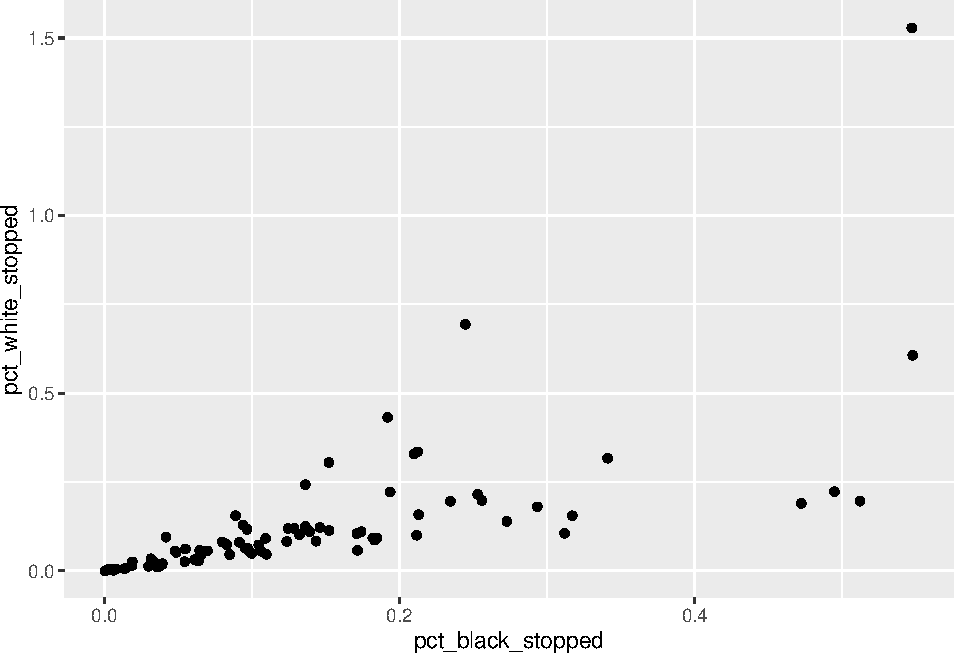
\includegraphics[width=0.7\linewidth]{R-data-viz_files/figure-latex/first-ggplot-1}

The \texttt{+} in the \textbf{\texttt{ggplot2}} package is particularly
useful because it allows you to modify existing \texttt{ggplot} objects.
This means you can easily set up plot ``templates'' and conveniently
explore different types of plots, so the above plot can also be
generated with code like this:

\begin{Shaded}
\begin{Highlighting}[]
\CommentTok{# Assign plot to a variable}
\NormalTok{MS_plot <-}\StringTok{ }\KeywordTok{ggplot}\NormalTok{(}\DataTypeTok{data =}\NormalTok{ MS_demographic, }\KeywordTok{aes}\NormalTok{(}\DataTypeTok{x =}\NormalTok{ pct_black_stopped, }\DataTypeTok{y =}\NormalTok{ pct_white_stopped))}

\CommentTok{# Draw the plot}
\NormalTok{MS_plot }\OperatorTok{+}\StringTok{ }\KeywordTok{geom_point}\NormalTok{()}
\end{Highlighting}
\end{Shaded}

Notes:

\begin{itemize}
\tightlist
\item
  Any parameters you set in the \texttt{ggplot()} function can be seen
  by any geom layers that you add (i.e., these are universal plot
  settings). This includes the x and y axis you set up in
  \texttt{aes()}.
\item
  Any parameters you set in the \texttt{geom\_*()} function are treated
  independently of (and override) the settings defined globally in the
  \texttt{ggplot()} function.
\item
  Geoms are plotted in the order they are added after each \texttt{+},
  that means geoms last added will display on top of prior geoms.
\item
  The \texttt{+} sign used to add layers \textbf{must be placed at the
  end of each line} containing a layer. If, instead, the \texttt{+} sign
  is added in the line before the other layer, \textbf{\texttt{ggplot2}}
  will not add the new layer and will return an error message.
\end{itemize}

\begin{Shaded}
\begin{Highlighting}[]
\CommentTok{# this is the correct syntax for adding layers}
\NormalTok{MS_plot }\OperatorTok{+}
\StringTok{  }\KeywordTok{geom_point}\NormalTok{()}

\CommentTok{# this will not add the new layer and will return an error message}
\NormalTok{MS_plot}
  \OperatorTok{+}\StringTok{ }\KeywordTok{geom_point}\NormalTok{()}
\end{Highlighting}
\end{Shaded}

To learn more about \textbf{\texttt{ggplot}} after the workshop, you may
want to check out this
\href{https://www.rstudio.com/wp-content/uploads/2016/11/ggplot2-cheatsheet-2.1.pdf}{cheatsheet
about \textbf{\texttt{ggplot}}}.

\section{Building your plots
iteratively}\label{building-your-plots-iteratively}

Building plots with ggplot can be of great help when you engage in
exploratory data analysis. It is typically an iterative process, where
you go back and forth between your data and their graphical
representation, which helps you in the process of getting to know your
data better.

Conveniently, \texttt{ggplot} works with pipes. The code below does the
same thing as above:

\begin{Shaded}
\begin{Highlighting}[]
\NormalTok{MS_demographic }\OperatorTok\StringTok{ }
\StringTok{  }\KeywordTok{ggplot}\NormalTok{(}\KeywordTok{aes}\NormalTok{(}\DataTypeTok{x =}\NormalTok{ pct_black_stopped, }\DataTypeTok{y =}\NormalTok{ pct_white_stopped)) }\OperatorTok{+}\StringTok{ }
\StringTok{  }\KeywordTok{geom_point}\NormalTok{() }
\end{Highlighting}
\end{Shaded}

We pipe the content of the table into \texttt{ggplot()}, so we can omit
the first (\texttt{data\ =} argument). Now let's use this to clean up a
few odd outliers in our data before we pass them to ggplot.

\begin{Shaded}
\begin{Highlighting}[]
\NormalTok{MS_demographic }\OperatorTok\StringTok{ }
\StringTok{  }\KeywordTok{filter}\NormalTok{(pct_white_stopped }\OperatorTok{<}\StringTok{ }\FloatTok{0.5} \OperatorTok{&}\StringTok{ }\NormalTok{pct_black_stopped }\OperatorTok{<}\StringTok{ }\FloatTok{0.5}\NormalTok{) }\OperatorTok\StringTok{ }
\StringTok{  }\KeywordTok{ggplot}\NormalTok{(}\KeywordTok{aes}\NormalTok{(}\DataTypeTok{x =}\NormalTok{ pct_black_stopped, }\DataTypeTok{y =}\NormalTok{ pct_white_stopped)) }\OperatorTok{+}\StringTok{ }
\StringTok{  }\KeywordTok{geom_point}\NormalTok{() }
\end{Highlighting}
\end{Shaded}

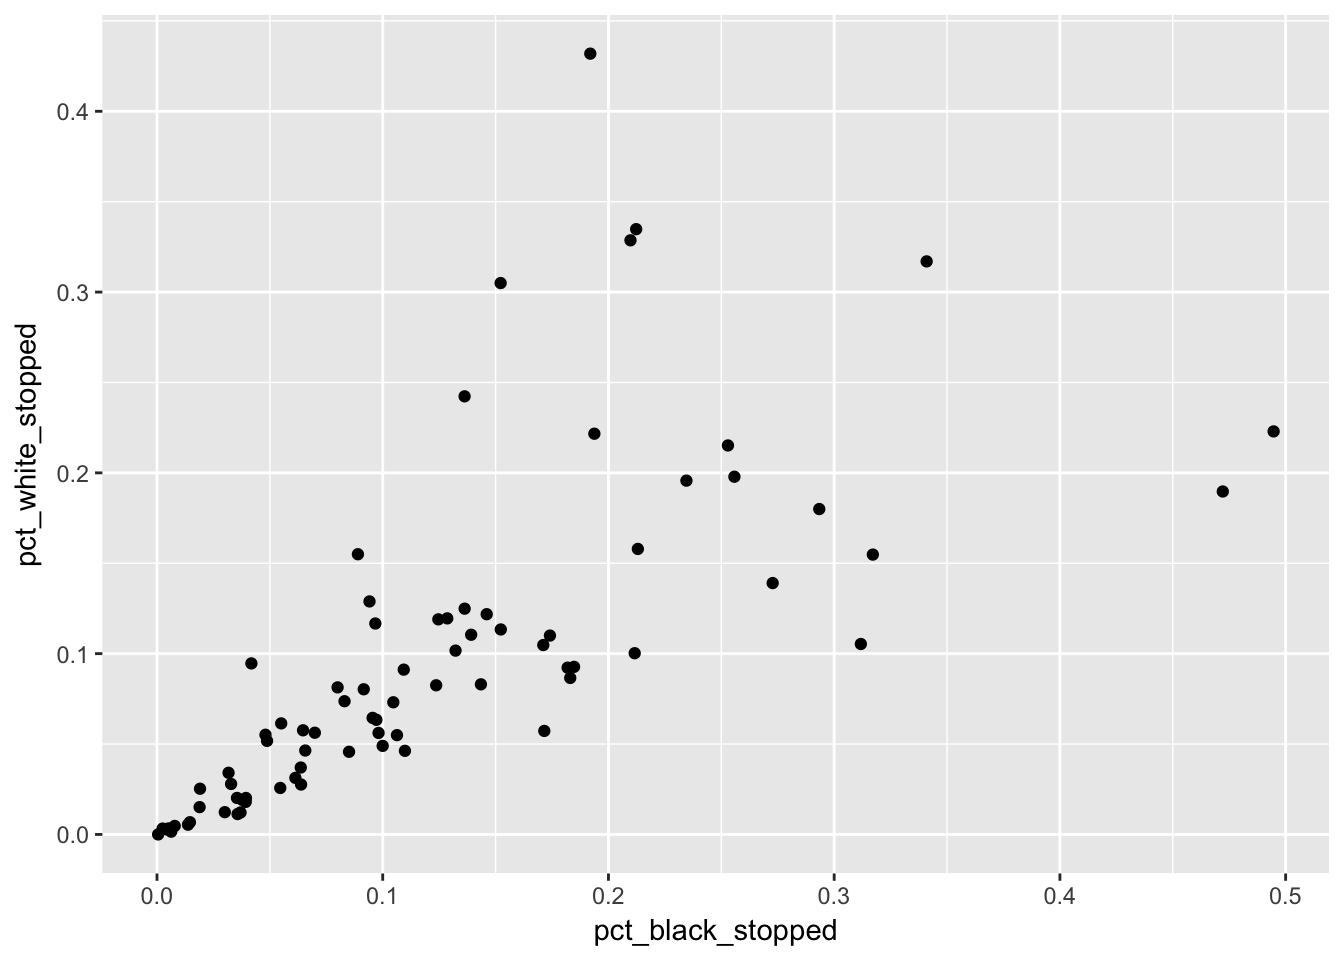
\includegraphics[width=0.7\linewidth]{R-data-viz_files/figure-latex/ggplot-with-filter-1}

Then we can start modifying this plot to extract more information from
it. For instance, we can add transparency (\texttt{alpha}) to avoid
overplotting:

\begin{Shaded}
\begin{Highlighting}[]
\NormalTok{MS_demographic }\OperatorTok\StringTok{ }
\StringTok{  }\KeywordTok{filter}\NormalTok{(pct_white_stopped }\OperatorTok{<}\StringTok{ }\FloatTok{0.5} \OperatorTok{&}\StringTok{ }\NormalTok{pct_black_stopped }\OperatorTok{<}\StringTok{ }\FloatTok{0.5}\NormalTok{) }\OperatorTok\StringTok{ }
\StringTok{  }\KeywordTok{ggplot}\NormalTok{(}\KeywordTok{aes}\NormalTok{(}\DataTypeTok{x =}\NormalTok{ pct_black_stopped, }\DataTypeTok{y =}\NormalTok{ pct_white_stopped)) }\OperatorTok{+}\StringTok{ }
\StringTok{  }\KeywordTok{geom_point}\NormalTok{(}\DataTypeTok{alpha =} \FloatTok{0.3}\NormalTok{)}
\end{Highlighting}
\end{Shaded}

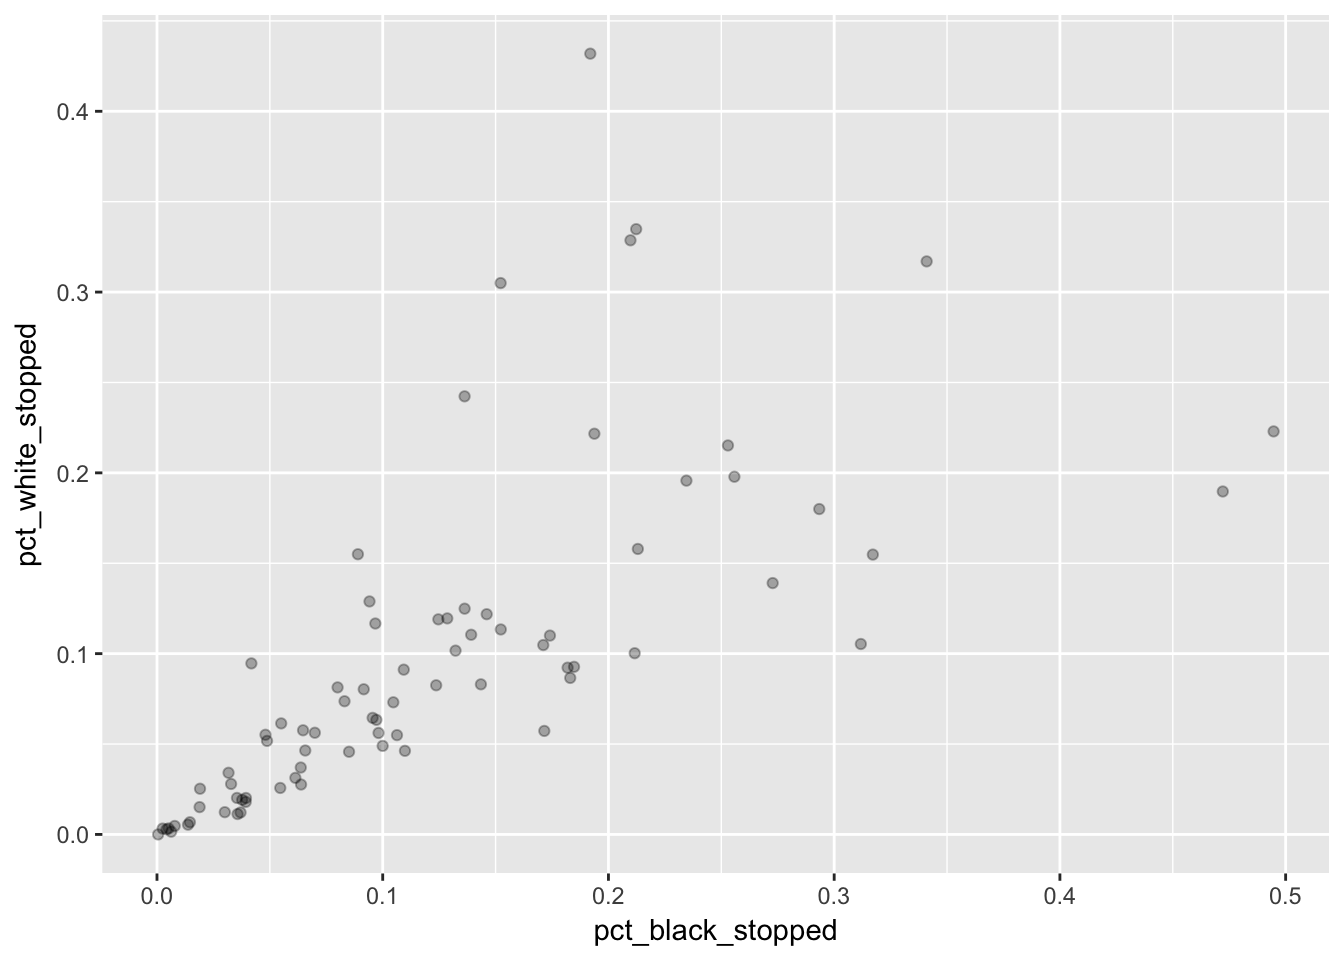
\includegraphics[width=0.7\linewidth]{R-data-viz_files/figure-latex/adding-transparency-1}

We can also add a color for all the points:

\begin{Shaded}
\begin{Highlighting}[]
\NormalTok{MS_demographic }\OperatorTok\StringTok{ }
\StringTok{  }\KeywordTok{filter}\NormalTok{(pct_white_stopped }\OperatorTok{<}\StringTok{ }\FloatTok{0.5} \OperatorTok{&}\StringTok{ }\NormalTok{pct_black_stopped }\OperatorTok{<}\StringTok{ }\FloatTok{0.5}\NormalTok{) }\OperatorTok\StringTok{ }
\StringTok{  }\KeywordTok{ggplot}\NormalTok{(}\KeywordTok{aes}\NormalTok{(}\DataTypeTok{x =}\NormalTok{ pct_black_stopped, }\DataTypeTok{y =}\NormalTok{ pct_white_stopped)) }\OperatorTok{+}\StringTok{ }
\StringTok{  }\KeywordTok{geom_point}\NormalTok{(}\DataTypeTok{alpha =} \FloatTok{0.3}\NormalTok{, }\DataTypeTok{color=} \StringTok{"blue"}\NormalTok{)}
\end{Highlighting}
\end{Shaded}

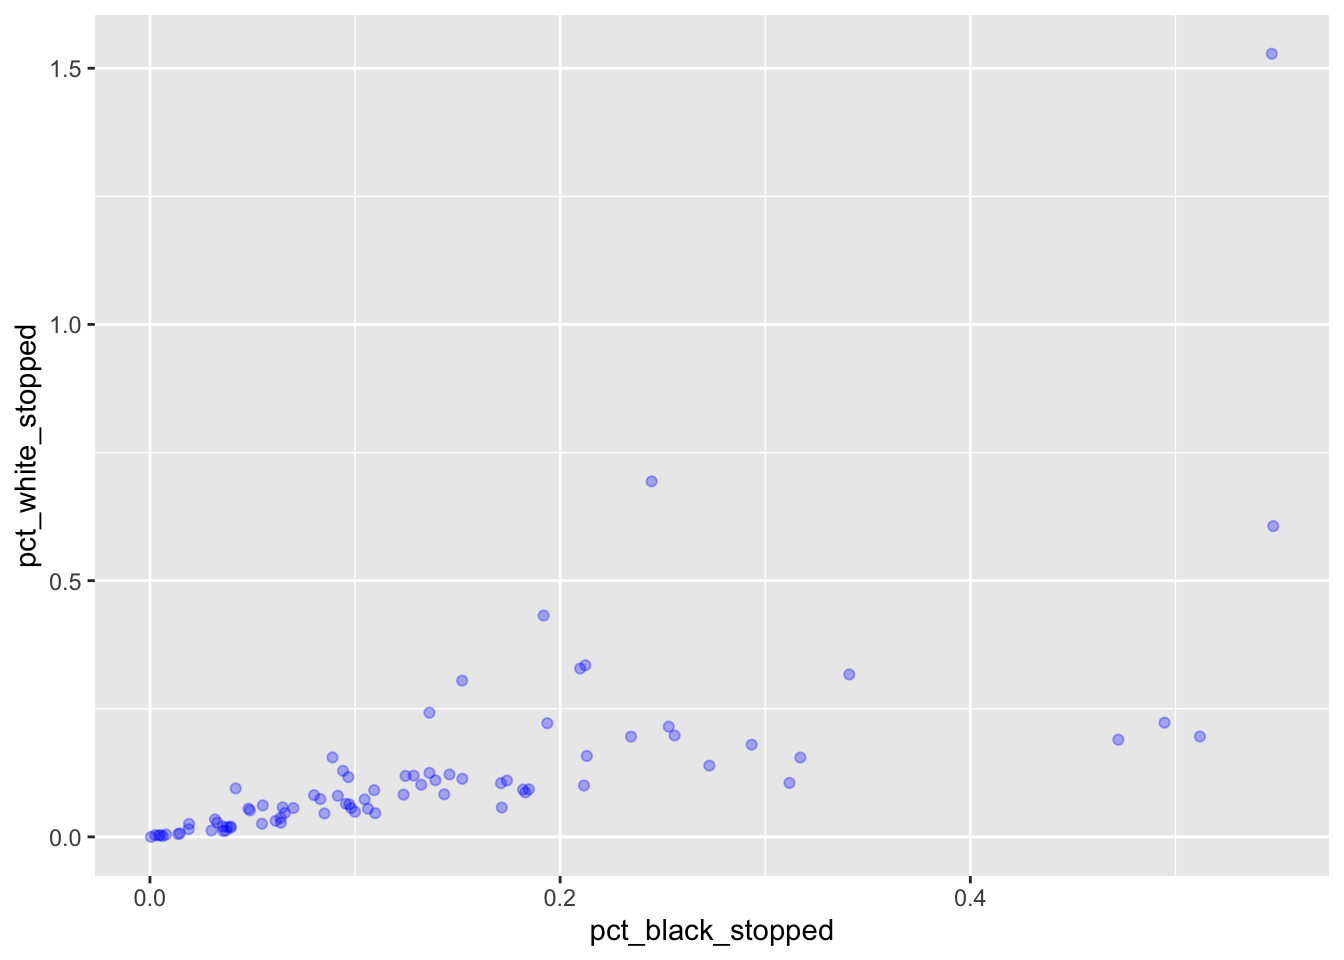
\includegraphics[width=0.7\linewidth]{R-data-viz_files/figure-latex/adding-color-1}

We can add another layer to the plot with \texttt{+}:

\begin{Shaded}
\begin{Highlighting}[]
\NormalTok{MS_demographic }\OperatorTok\StringTok{ }
\StringTok{  }\KeywordTok{filter}\NormalTok{(pct_white_stopped }\OperatorTok{<}\StringTok{ }\FloatTok{0.5} \OperatorTok{&}\StringTok{ }\NormalTok{pct_black_stopped }\OperatorTok{<}\StringTok{ }\FloatTok{0.5}\NormalTok{) }\OperatorTok\StringTok{ }
\StringTok{  }\KeywordTok{ggplot}\NormalTok{(}\KeywordTok{aes}\NormalTok{(}\DataTypeTok{x =}\NormalTok{ pct_black_stopped, }\DataTypeTok{y =}\NormalTok{ pct_white_stopped)) }\OperatorTok{+}\StringTok{ }
\StringTok{  }\KeywordTok{geom_point}\NormalTok{(}\DataTypeTok{alpha =} \FloatTok{0.3}\NormalTok{, }\DataTypeTok{color=} \StringTok{"blue"}\NormalTok{) }\OperatorTok{+}
\StringTok{  }\KeywordTok{geom_abline}\NormalTok{(}\DataTypeTok{intercept =} \DecValTok{0}\NormalTok{)}
\end{Highlighting}
\end{Shaded}

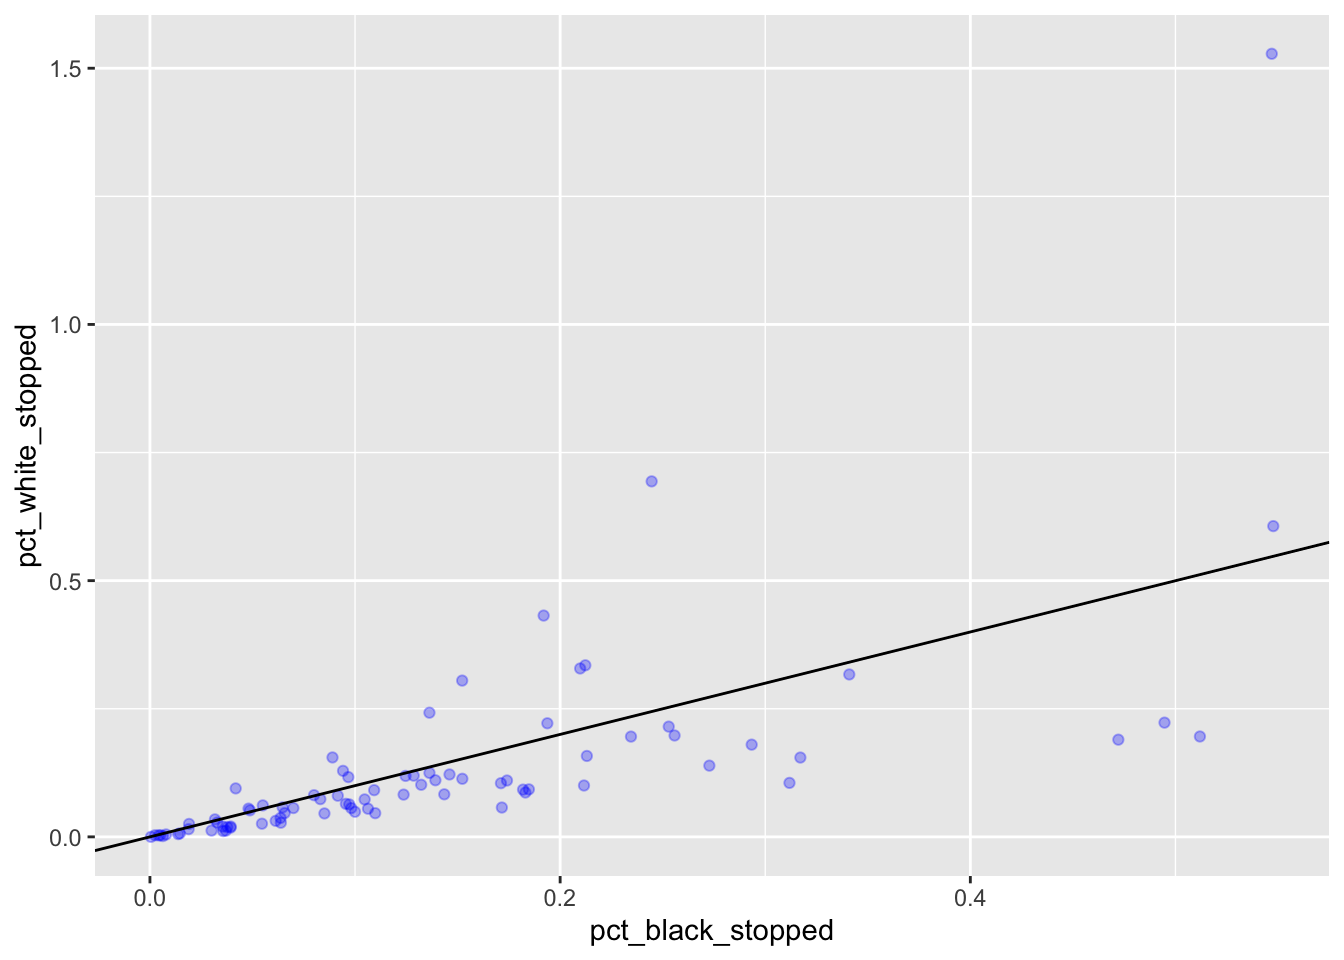
\includegraphics[width=0.7\linewidth]{R-data-viz_files/figure-latex/add-abline-1}

If we wanted to ``zoom'' into the plot, we could filter to a smaller
range of values before passing them to ggplot, but we can also tell
ggplot to only plot the x and y values for certain ranges. For this we
use \texttt{scale\_x\_continuous} and \texttt{scale\_y\_continuous}. You
will receive a message from ggplot telling you how many rows it has
removed from the plot.

\begin{Shaded}
\begin{Highlighting}[]
\NormalTok{MS_demographic }\OperatorTok\StringTok{ }
\StringTok{  }\KeywordTok{filter}\NormalTok{(pct_white_stopped }\OperatorTok{<}\StringTok{ }\FloatTok{0.5} \OperatorTok{&}\StringTok{ }\NormalTok{pct_black_stopped }\OperatorTok{<}\StringTok{ }\FloatTok{0.5}\NormalTok{) }\OperatorTok\StringTok{ }
\StringTok{  }\KeywordTok{ggplot}\NormalTok{(}\KeywordTok{aes}\NormalTok{(}\DataTypeTok{x =}\NormalTok{ pct_black_stopped, }\DataTypeTok{y =}\NormalTok{ pct_white_stopped)) }\OperatorTok{+}\StringTok{ }
\StringTok{  }\KeywordTok{geom_point}\NormalTok{(}\DataTypeTok{alpha =} \FloatTok{0.3}\NormalTok{, }\DataTypeTok{color=} \StringTok{"blue"}\NormalTok{) }\OperatorTok{+}
\StringTok{  }\KeywordTok{geom_abline}\NormalTok{(}\DataTypeTok{intercept =} \DecValTok{0}\NormalTok{) }\OperatorTok{+}\StringTok{ }
\StringTok{  }\KeywordTok{scale_x_continuous}\NormalTok{(}\DataTypeTok{limits =} \KeywordTok{c}\NormalTok{(}\DecValTok{0}\NormalTok{, }\FloatTok{0.1}\NormalTok{)) }\OperatorTok{+}
\StringTok{  }\KeywordTok{scale_y_continuous}\NormalTok{(}\DataTypeTok{limits =} \KeywordTok{c}\NormalTok{(}\DecValTok{0}\NormalTok{, }\FloatTok{0.1}\NormalTok{)) }
\end{Highlighting}
\end{Shaded}

\begin{verbatim}
#> Warning: Removed 40 rows containing missing values (geom_point).
\end{verbatim}

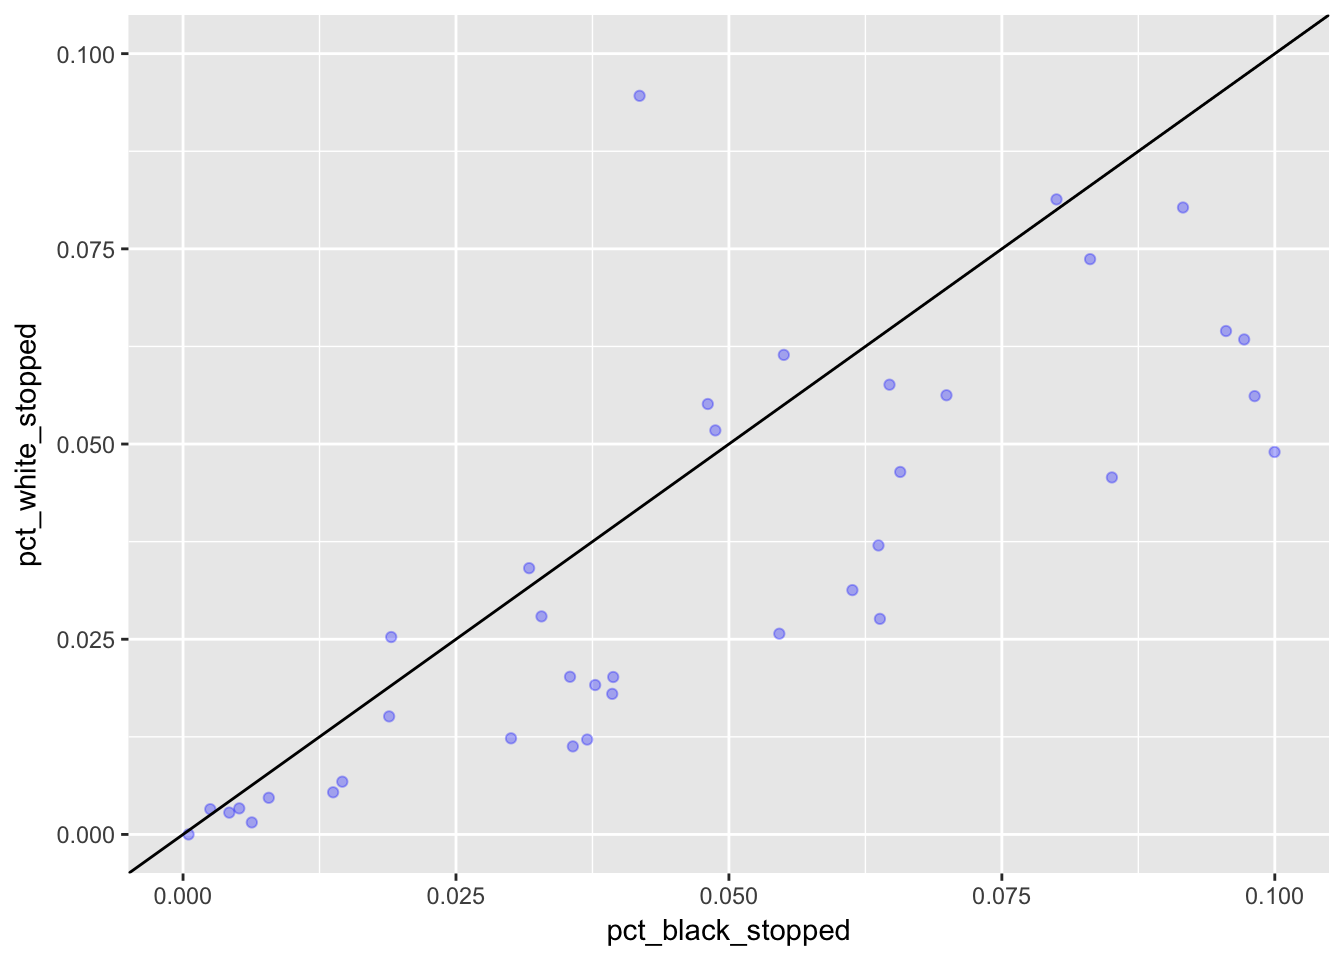
\includegraphics[width=0.7\linewidth]{R-data-viz_files/figure-latex/zoom-in-1}

\begin{quote}
Challenge

Modify the plot above to display different color for both points and
abline, and show a different range of data. How might you change the
size of the dots?
\end{quote}

\section{Barplot}\label{barplot}

There are two types of bar charts in ggplot, \texttt{geom\_bar} and
\texttt{geom\_col}. \texttt{geom\_bar} makes the height of the bar
proportional to the number of cases in each group and counts the number
of cases at each x position.

If we wanted to see how many violations we have of each type could say:

\begin{Shaded}
\begin{Highlighting}[]
\KeywordTok{ggplot}\NormalTok{(trafficstops, }\KeywordTok{aes}\NormalTok{(violation)) }\OperatorTok{+}\StringTok{ }
\StringTok{  }\KeywordTok{geom_bar}\NormalTok{()}
\end{Highlighting}
\end{Shaded}

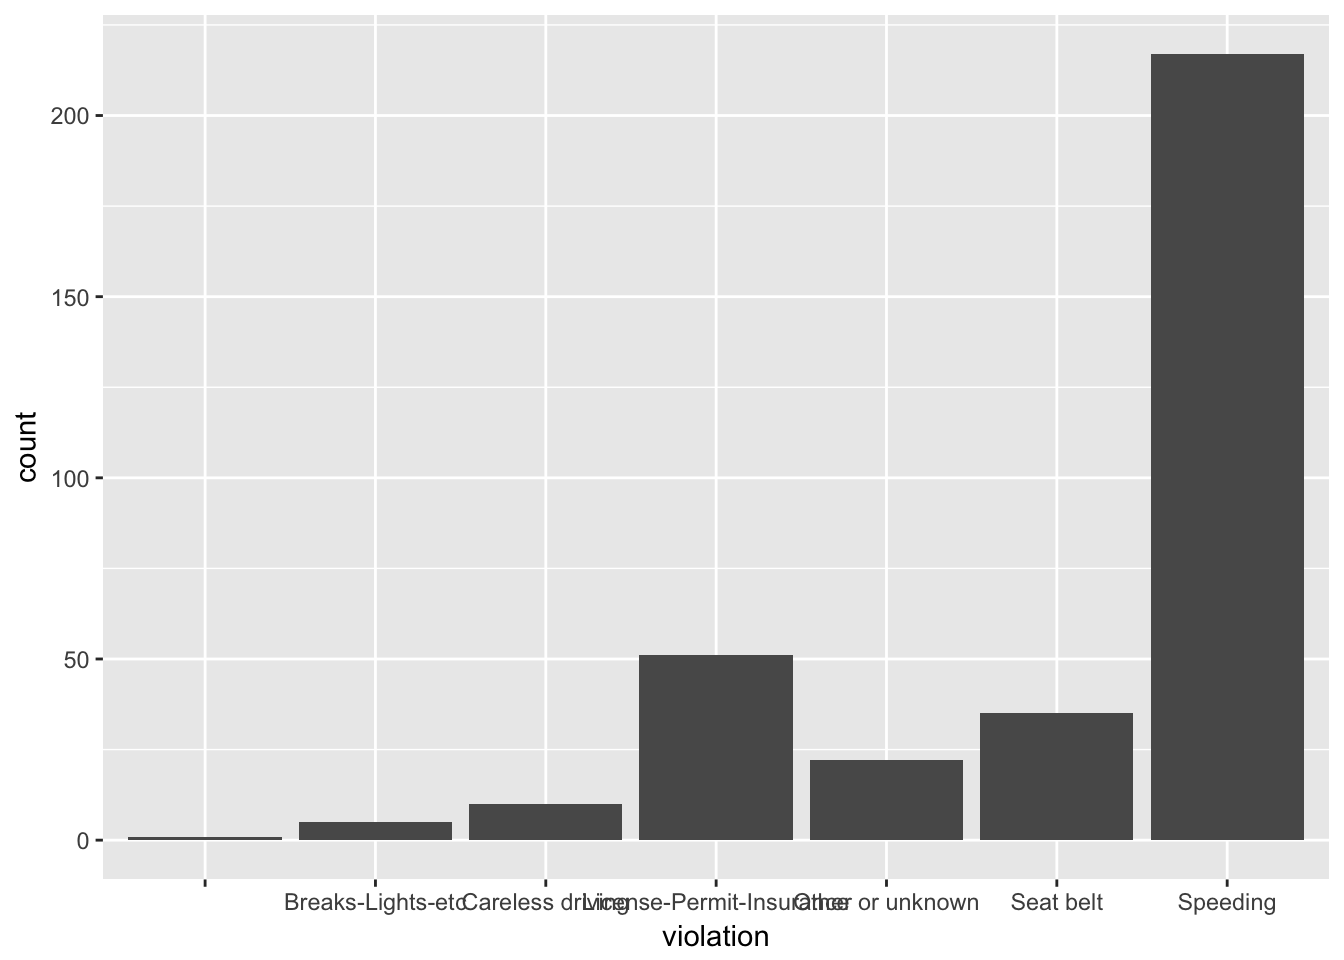
\includegraphics[width=0.7\linewidth]{R-data-viz_files/figure-latex/simple-bar-1}

As we have seen we could color the bars, but instead of \texttt{color}
we use \texttt{fill}. (What happens when you use \texttt{color}?)

\begin{Shaded}
\begin{Highlighting}[]
\KeywordTok{ggplot}\NormalTok{(trafficstops, }\KeywordTok{aes}\NormalTok{(violation)) }\OperatorTok{+}\StringTok{ }
\StringTok{  }\KeywordTok{geom_bar}\NormalTok{(}\DataTypeTok{fill =} \StringTok{"green"}\NormalTok{)}
\end{Highlighting}
\end{Shaded}

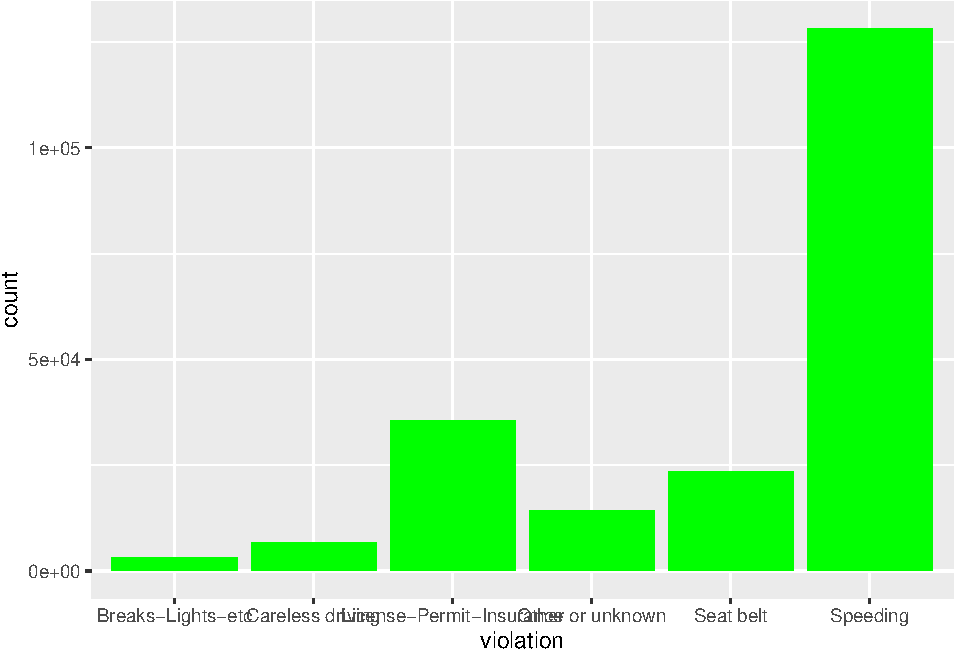
\includegraphics[width=0.7\linewidth]{R-data-viz_files/figure-latex/color-bar-simple-1}

Instead of coloring everything the same we could also color by another
category, say gender. For this we have to set the parameter within the
\texttt{aes()} function, which takes care of mapping the values to
different colors:

\begin{Shaded}
\begin{Highlighting}[]
\KeywordTok{ggplot}\NormalTok{(trafficstops, }\KeywordTok{aes}\NormalTok{(violation)) }\OperatorTok{+}\StringTok{ }
\StringTok{  }\KeywordTok{geom_bar}\NormalTok{(}\KeywordTok{aes}\NormalTok{(}\DataTypeTok{fill =}\NormalTok{ driver_gender))}
\end{Highlighting}
\end{Shaded}

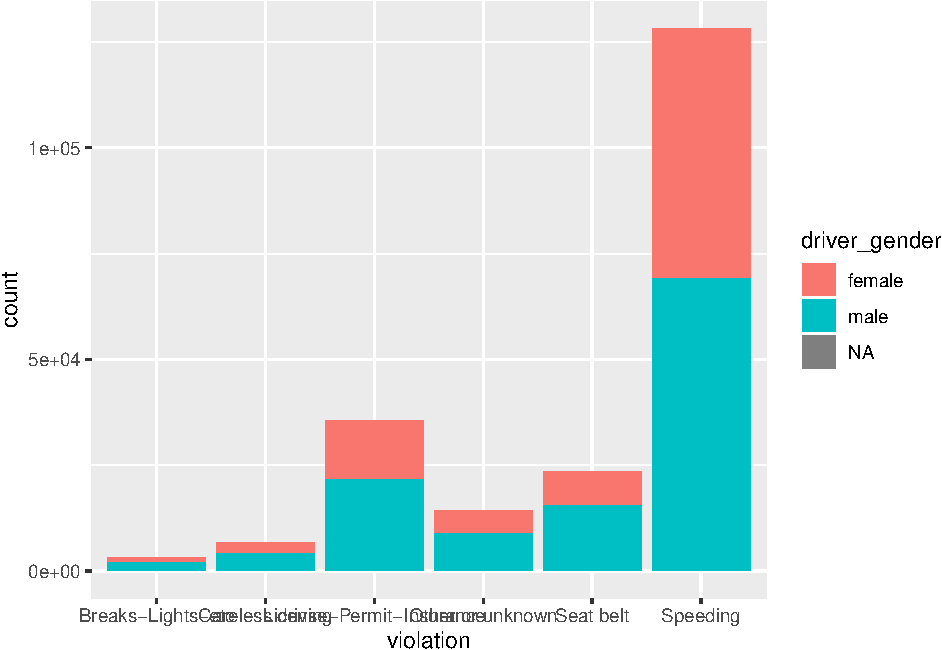
\includegraphics[width=0.7\linewidth]{R-data-viz_files/figure-latex/color-bar-gender-1}

If we wanted to see the proportions within each category we can tell
ggplot to stretch the bars between 0 and 1, we can set the position
parameter to `fill':

\begin{Shaded}
\begin{Highlighting}[]
\KeywordTok{ggplot}\NormalTok{(trafficstops, }\KeywordTok{aes}\NormalTok{(violation)) }\OperatorTok{+}\StringTok{ }
\StringTok{  }\KeywordTok{geom_bar}\NormalTok{(}\KeywordTok{aes}\NormalTok{(}\DataTypeTok{fill =}\NormalTok{ driver_gender), }\DataTypeTok{position =} \StringTok{"fill"}\NormalTok{)}
\end{Highlighting}
\end{Shaded}

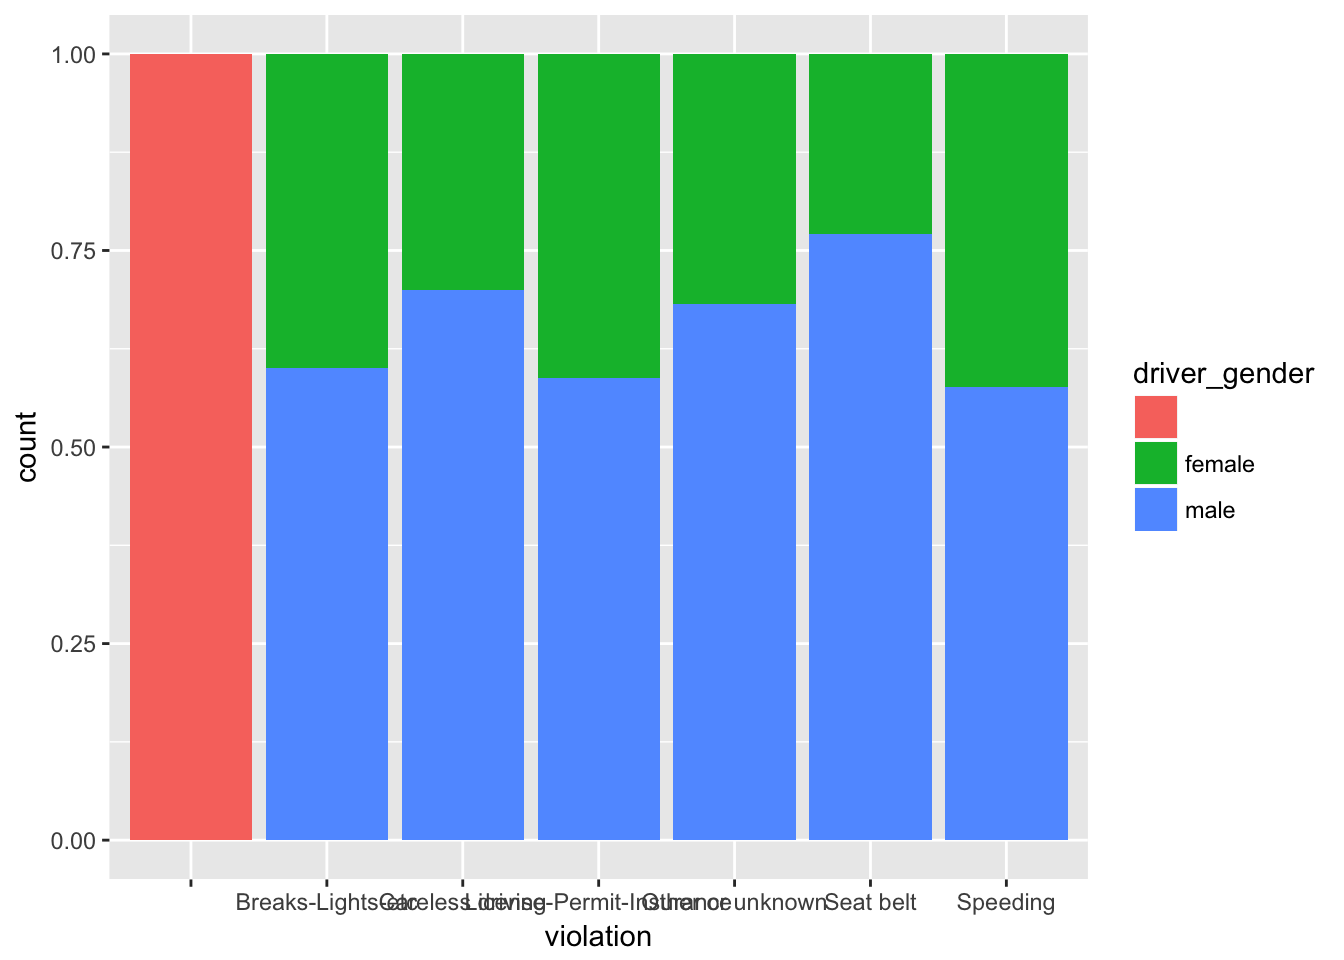
\includegraphics[width=0.7\linewidth]{R-data-viz_files/figure-latex/color-bar-stretch-1}

The other type of barchart, \texttt{geom\_col}, is used if you want the
heights of the bars to represent values in the data. It leaves the data
as is. For example, we can use \texttt{geom\_col} for a different way of
visualizing the data shown in the scatterplot above. For readability I
have also flipped the coordinates:

\begin{Shaded}
\begin{Highlighting}[]
\NormalTok{MS_demographic }\OperatorTok\StringTok{   }
\StringTok{  }\KeywordTok{filter}\NormalTok{(pct_white_stopped }\OperatorTok{<}\StringTok{ }\FloatTok{0.5} \OperatorTok{&}\StringTok{ }\NormalTok{pct_black_stopped }\OperatorTok{<}\StringTok{ }\FloatTok{0.5}\NormalTok{) }\OperatorTok
\StringTok{  }\KeywordTok{ggplot}\NormalTok{(}\KeywordTok{aes}\NormalTok{(}\DataTypeTok{x =}\NormalTok{ county_name, }\DataTypeTok{y =}\NormalTok{ pct_white_stopped }\OperatorTok{-}\StringTok{ }\NormalTok{pct_black_stopped)) }\OperatorTok{+}\StringTok{ }
\StringTok{    }\KeywordTok{geom_col}\NormalTok{() }\OperatorTok{+}\StringTok{ }
\StringTok{    }\KeywordTok{coord_flip}\NormalTok{()}
\end{Highlighting}
\end{Shaded}

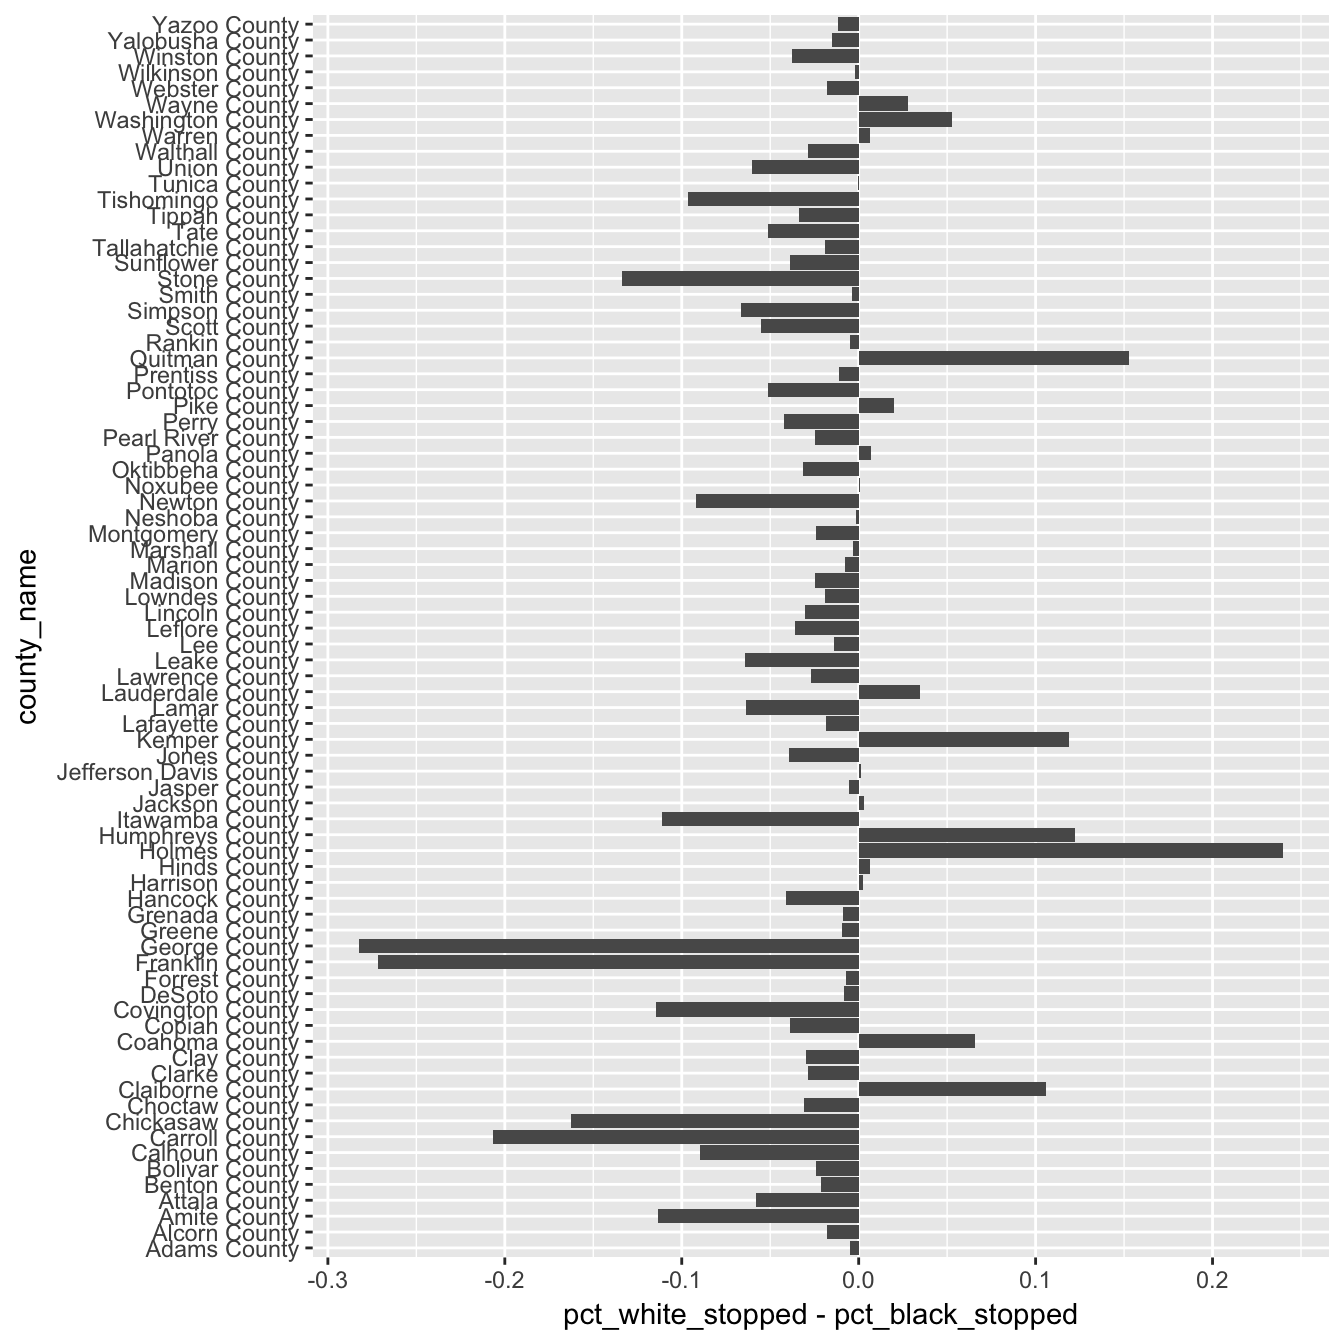
\includegraphics{R-data-viz_files/figure-latex/demograph-barplot-1.pdf}

\begin{quote}
Challenge

Make a barplot that shows for each race the proportion of stops for male
and female drivers. How could you get rid of the NAs?
\end{quote}

\section{Boxplot}\label{boxplot}

For this segment let's extract and work with the stops for Chickasaw
County only.

\begin{Shaded}
\begin{Highlighting}[]
\NormalTok{Chickasaw_stops <-}\StringTok{ }\KeywordTok{filter}\NormalTok{(trafficstops, county_name }\OperatorTok{==}\StringTok{ "Chickasaw County"}\NormalTok{)}
\end{Highlighting}
\end{Shaded}

We can use boxplots to visualize the distribution of driver age within
each violation:

\begin{Shaded}
\begin{Highlighting}[]
\KeywordTok{ggplot}\NormalTok{(}\DataTypeTok{data =}\NormalTok{ Chickasaw_stops, }\KeywordTok{aes}\NormalTok{(}\DataTypeTok{x =}\NormalTok{ violation, }\DataTypeTok{y =}\NormalTok{ driver_age)) }\OperatorTok{+}
\StringTok{    }\KeywordTok{geom_boxplot}\NormalTok{()}
\end{Highlighting}
\end{Shaded}

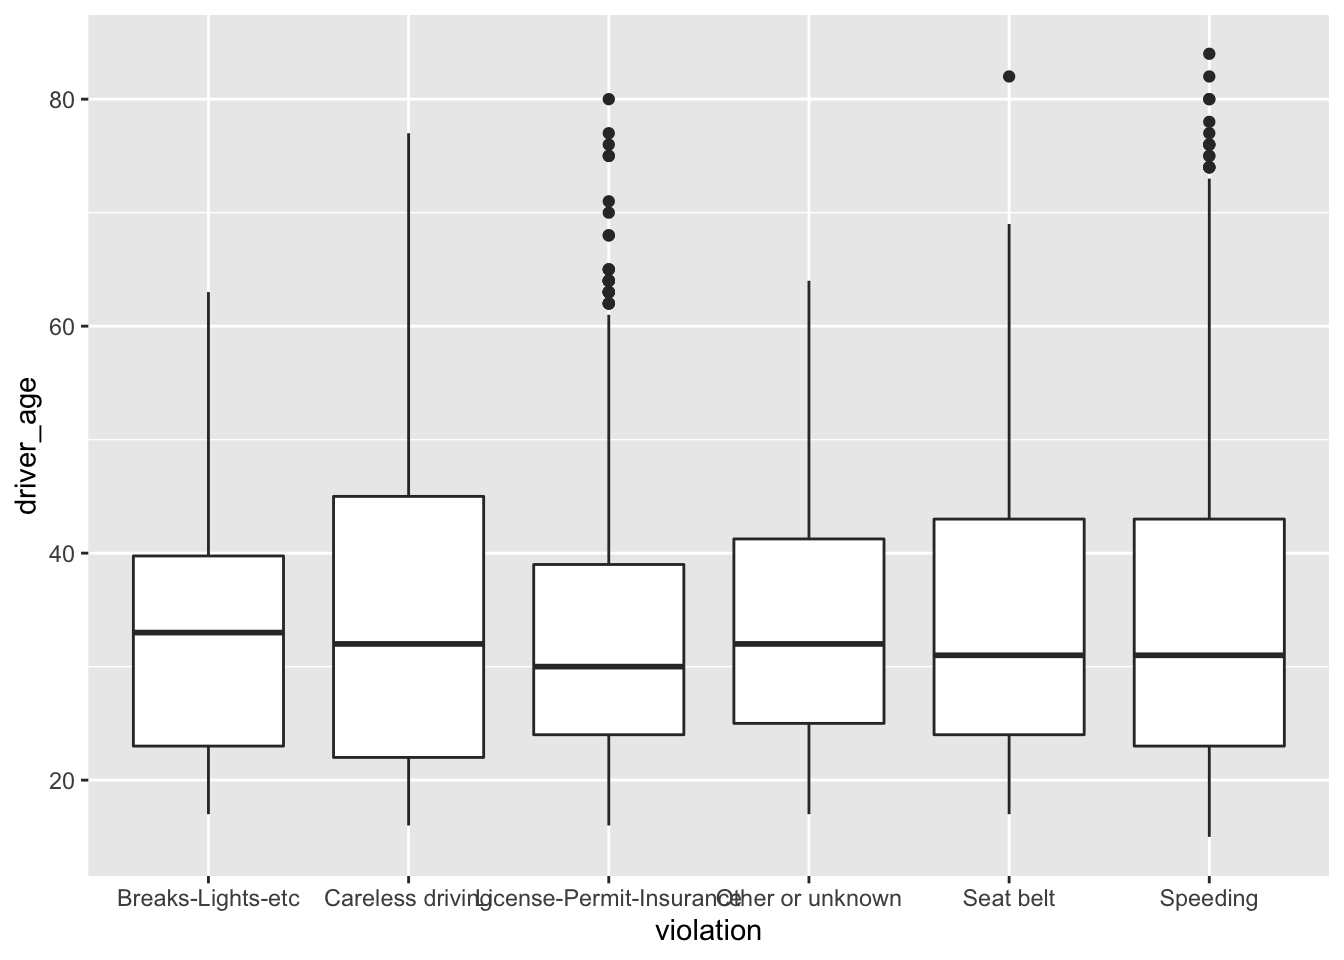
\includegraphics[width=0.7\linewidth]{R-data-viz_files/figure-latex/boxplot-1}

By adding points to boxplot, we can have a better idea of the number of
measurements and of their distribution.

\begin{Shaded}
\begin{Highlighting}[]
\KeywordTok{ggplot}\NormalTok{(}\DataTypeTok{data =}\NormalTok{ Chickasaw_stops, }\KeywordTok{aes}\NormalTok{(}\DataTypeTok{x =}\NormalTok{ violation, }\DataTypeTok{y =}\NormalTok{ driver_age)) }\OperatorTok{+}
\StringTok{    }\KeywordTok{geom_boxplot}\NormalTok{() }\OperatorTok{+}
\StringTok{    }\KeywordTok{geom_jitter}\NormalTok{()}
\end{Highlighting}
\end{Shaded}

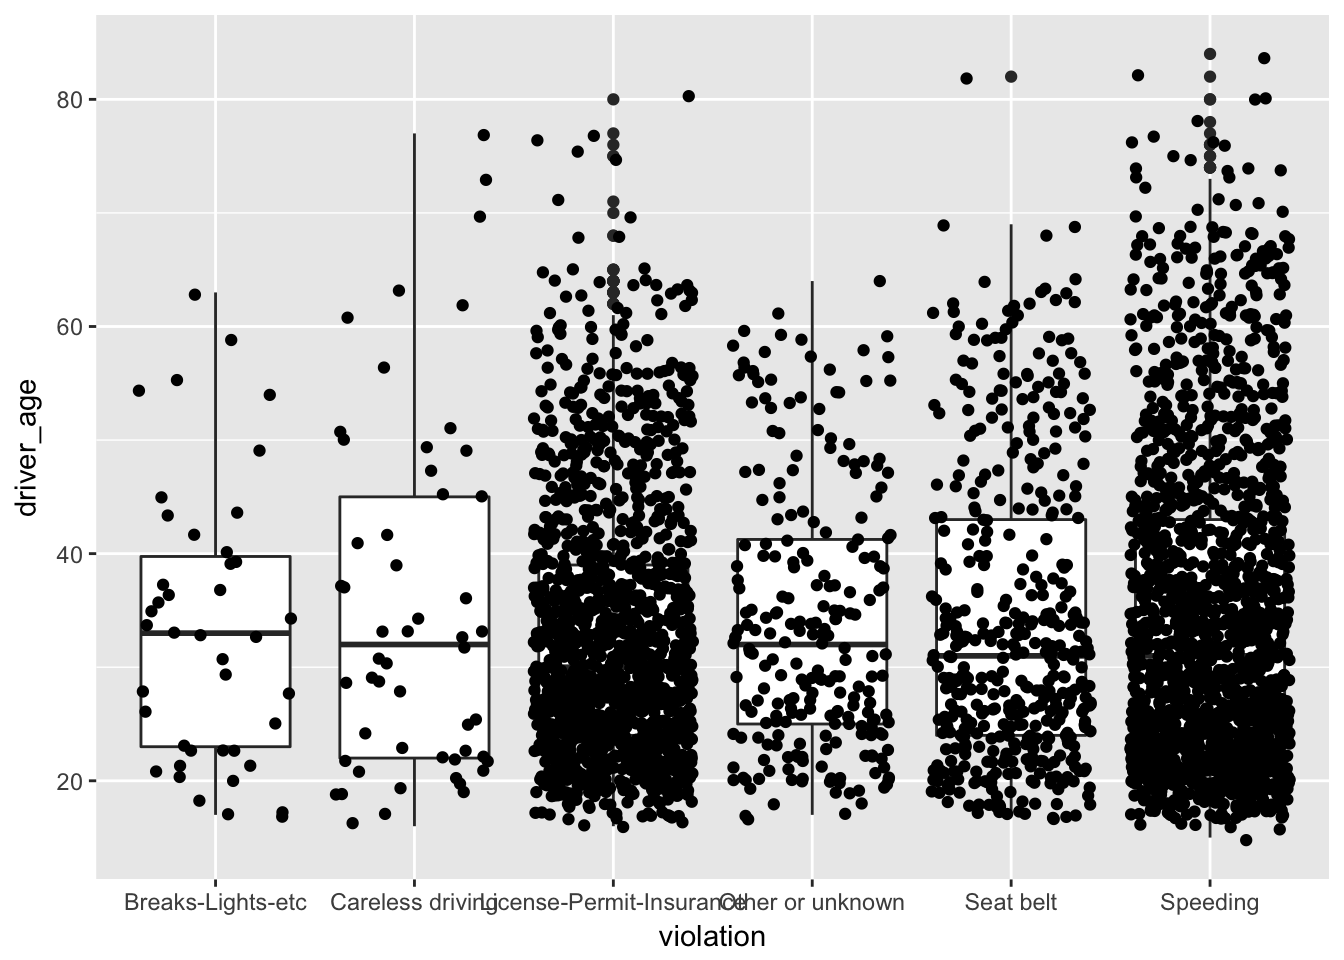
\includegraphics[width=0.7\linewidth]{R-data-viz_files/figure-latex/boxplot-with-jitter-1}

That looks quite messy. Let's clean it up by using the \texttt{alpha}
parameter to make the dots more transparent and also change their color:

\begin{Shaded}
\begin{Highlighting}[]
\KeywordTok{ggplot}\NormalTok{(}\DataTypeTok{data =}\NormalTok{ Chickasaw_stops, }\KeywordTok{aes}\NormalTok{(}\DataTypeTok{x =}\NormalTok{ violation, }\DataTypeTok{y =}\NormalTok{ driver_age)) }\OperatorTok{+}
\StringTok{    }\KeywordTok{geom_boxplot}\NormalTok{() }\OperatorTok{+}
\StringTok{    }\KeywordTok{geom_jitter}\NormalTok{(}\DataTypeTok{alpha =} \FloatTok{0.5}\NormalTok{, }\DataTypeTok{color =} \StringTok{"tomato"}\NormalTok{)}
\end{Highlighting}
\end{Shaded}

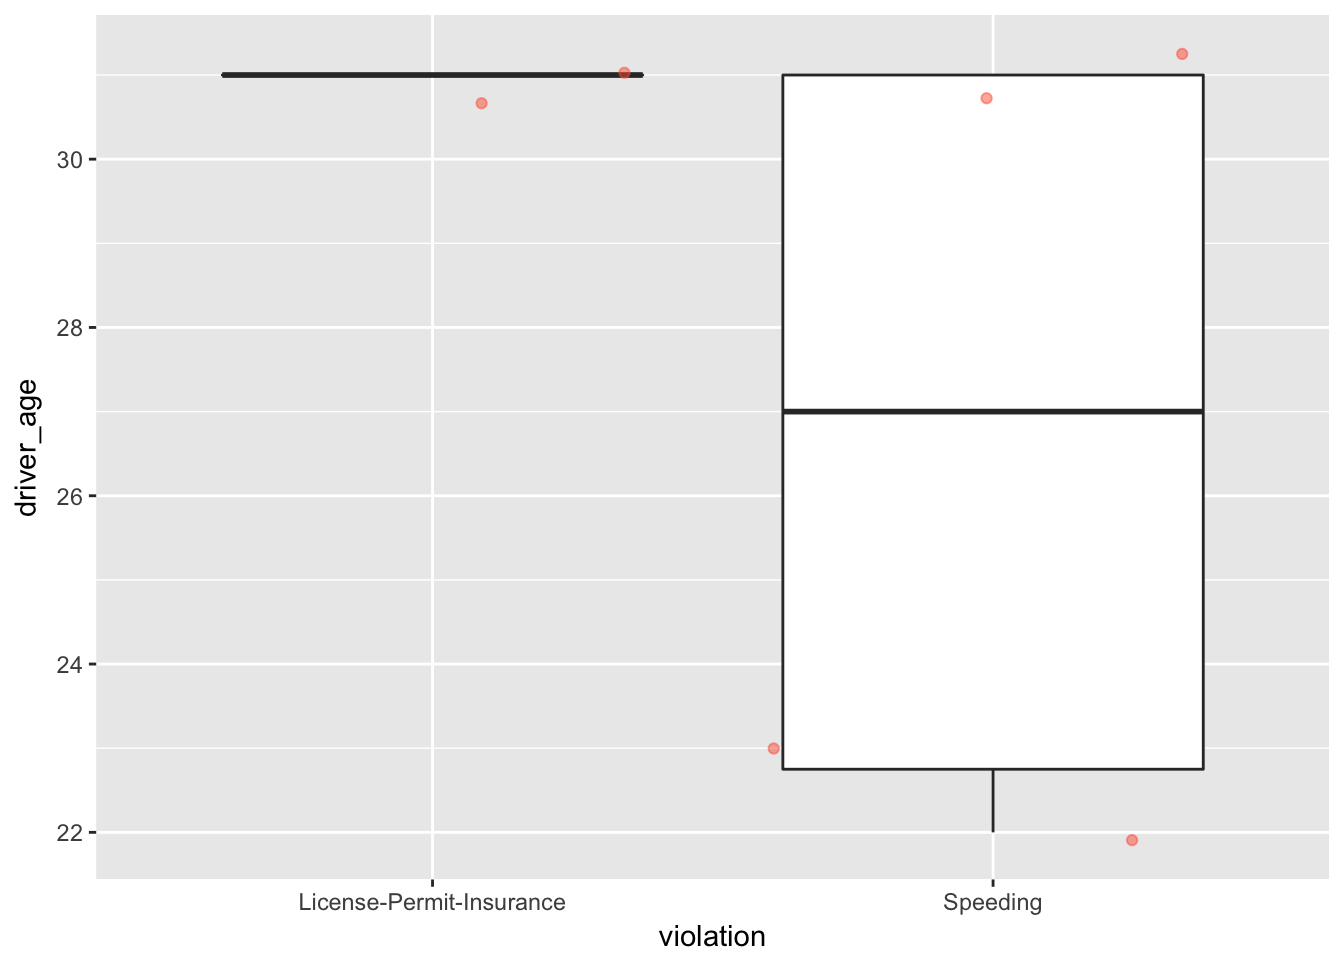
\includegraphics[width=0.7\linewidth]{R-data-viz_files/figure-latex/boxplot-with-jitter-transparent-1}

Notice how the boxplot layer is behind the jitter layer. We will change
the plotting order to keep the boxplot visible.

\begin{Shaded}
\begin{Highlighting}[]
\KeywordTok{ggplot}\NormalTok{(}\DataTypeTok{data =}\NormalTok{ Chickasaw_stops, }\KeywordTok{aes}\NormalTok{(}\DataTypeTok{x =}\NormalTok{ violation, }\DataTypeTok{y =}\NormalTok{ driver_age)) }\OperatorTok{+}
\StringTok{    }\KeywordTok{geom_jitter}\NormalTok{(}\DataTypeTok{alpha =} \FloatTok{0.1}\NormalTok{, }\DataTypeTok{color =} \StringTok{"tomato"}\NormalTok{) }\OperatorTok{+}\StringTok{ }
\StringTok{    }\KeywordTok{geom_boxplot}\NormalTok{()}
\end{Highlighting}
\end{Shaded}

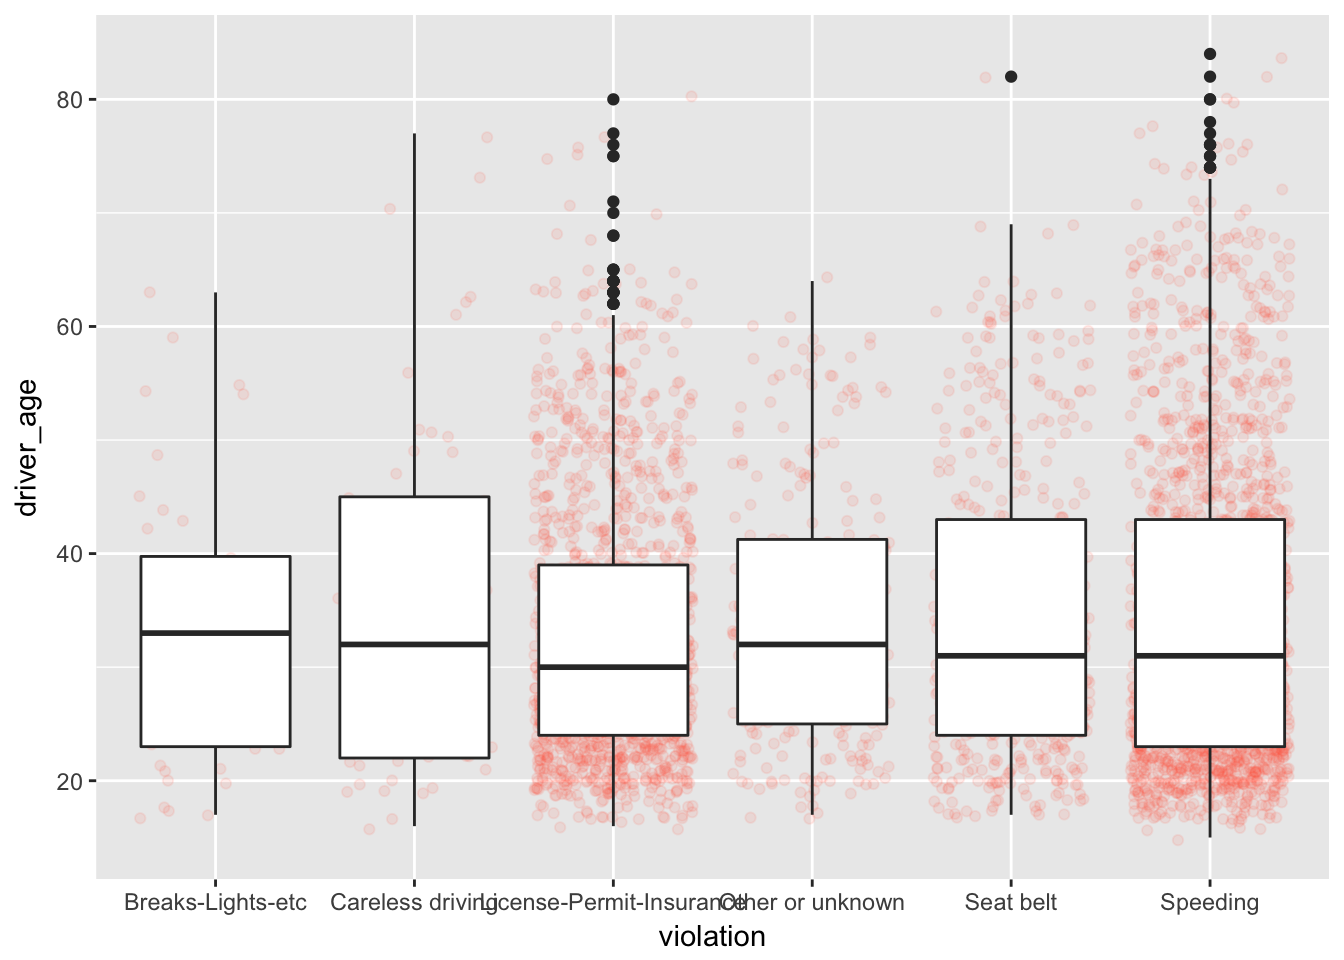
\includegraphics[width=0.7\linewidth]{R-data-viz_files/figure-latex/boxplot-with-jitter-reordered-1}

And finally we will change the transparency of the box plot so it does
not cover the points:

\begin{Shaded}
\begin{Highlighting}[]
\KeywordTok{ggplot}\NormalTok{(}\DataTypeTok{data =}\NormalTok{ Chickasaw_stops, }\KeywordTok{aes}\NormalTok{(}\DataTypeTok{x =}\NormalTok{ violation, }\DataTypeTok{y =}\NormalTok{ driver_age)) }\OperatorTok{+}
\StringTok{    }\KeywordTok{geom_jitter}\NormalTok{(}\DataTypeTok{alpha =} \FloatTok{0.1}\NormalTok{, }\DataTypeTok{color =} \StringTok{"tomato"}\NormalTok{) }\OperatorTok{+}
\StringTok{    }\KeywordTok{geom_boxplot}\NormalTok{(}\DataTypeTok{alpha =} \DecValTok{0}\NormalTok{)  }
\end{Highlighting}
\end{Shaded}

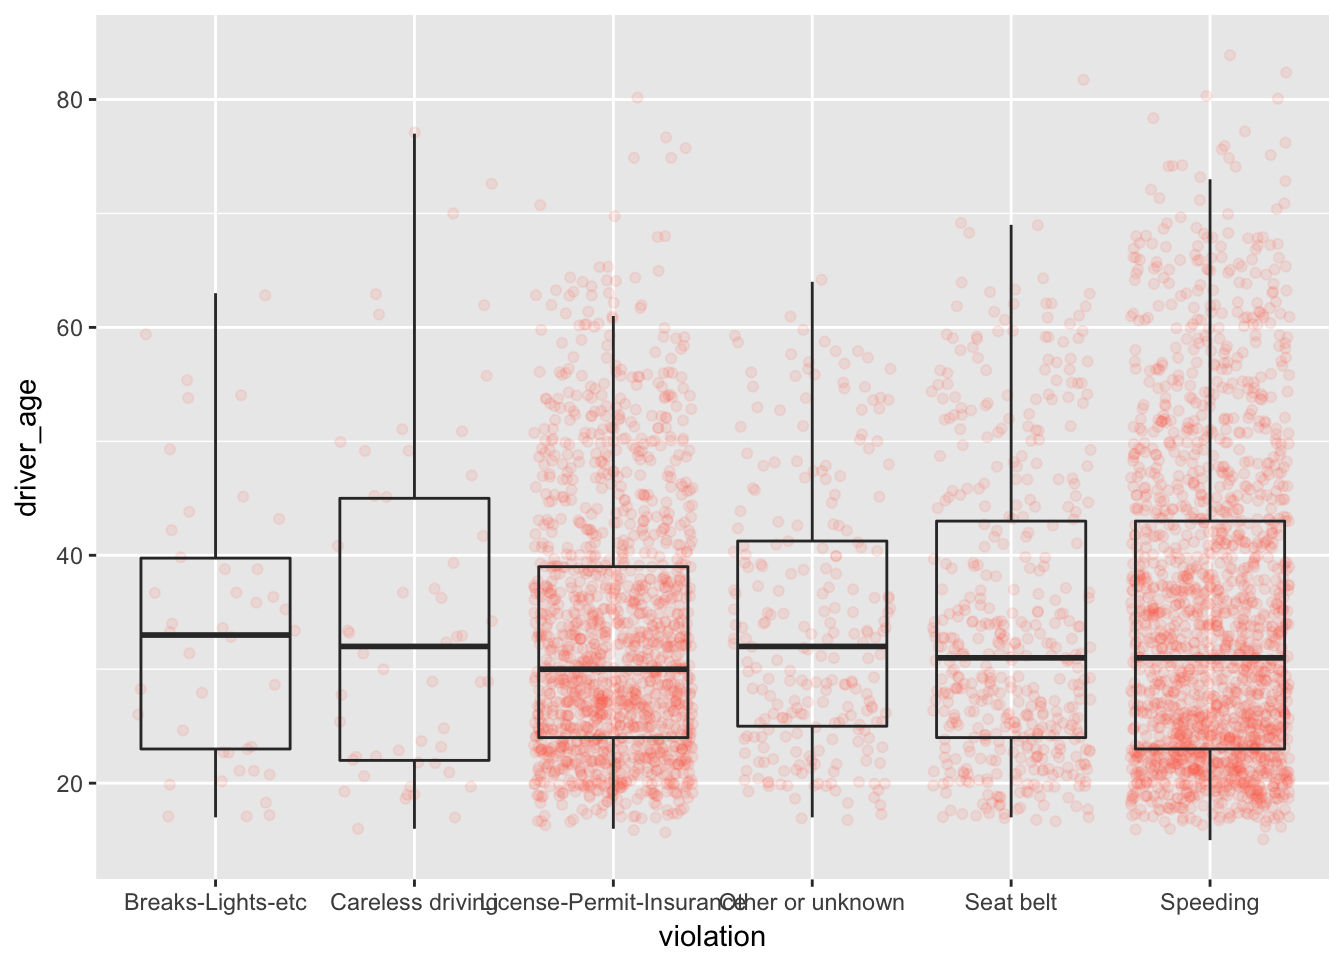
\includegraphics[width=0.7\linewidth]{R-data-viz_files/figure-latex/boxplot-with-jitter-clean-1}

\begin{quote}
Challenge

Boxplots are useful summaries, but hide the \emph{shape} of the
distribution. For example, if there is a bimodal distribution, it would
not be observed with a boxplot. An alternative to the boxplot is the
violin plot (sometimes known as a beanplot), where the shape (of the
density of points) is drawn.

\begin{itemize}
\tightlist
\item
  Replace the box plot with a violin plot; see \texttt{geom\_violin()}.
\end{itemize}

So far, we've looked at the distribution of age within violations Try
making a new plot to explore the distribution of age for another
variable:

\begin{itemize}
\tightlist
\item
  Create the age box plot for \texttt{driver\_race}. Overlay the boxplot
  layer on a jitter layer to show actual measurements.
\end{itemize}
\end{quote}

\section{Plotting time series data}\label{plotting-time-series-data}

To make things a little easer we first convert the date column we plan
to use to Date format.

\begin{Shaded}
\begin{Highlighting}[]
\KeywordTok{library}\NormalTok{(lubridate)}
\KeywordTok{class}\NormalTok{(trafficstops}\OperatorTok{$}\NormalTok{stop_date)}
\NormalTok{trafficstops}\OperatorTok{$}\NormalTok{stop_date <-}\StringTok{ }\KeywordTok{ymd}\NormalTok{(trafficstops}\OperatorTok{$}\NormalTok{stop_date)}
\KeywordTok{class}\NormalTok{(trafficstops}\OperatorTok{$}\NormalTok{stop_date)}
\end{Highlighting}
\end{Shaded}

Let's calculate number of violation per weekday. For better
understanding we will label the weekdays. First we need to group the
data and count records within each group:

\begin{Shaded}
\begin{Highlighting}[]
\NormalTok{trafficstops }\OperatorTok\StringTok{ }
\StringTok{  }\KeywordTok{mutate}\NormalTok{(}\DataTypeTok{wk_day =} \KeywordTok{wday}\NormalTok{(stop_date, }\DataTypeTok{label =} \OtherTok{TRUE}\NormalTok{)) }\OperatorTok\StringTok{  }
\StringTok{  }\KeywordTok{group_by}\NormalTok{(wk_day, violation) }\OperatorTok
\StringTok{  }\NormalTok{tally}
\end{Highlighting}
\end{Shaded}

Timelapse data can be visualized as a line plot (with -- you guessed it
-- \texttt{geom\_line()}) mapping the days to the x axis and counts to
the y axis. So we pipe the output from above into ggplot like this:

\begin{Shaded}
\begin{Highlighting}[]
\NormalTok{trafficstops }\OperatorTok\StringTok{ }
\StringTok{  }\KeywordTok{mutate}\NormalTok{(}\DataTypeTok{wk_day =} \KeywordTok{wday}\NormalTok{(stop_date, }\DataTypeTok{label =} \OtherTok{TRUE}\NormalTok{)) }\OperatorTok\StringTok{  }
\StringTok{  }\KeywordTok{group_by}\NormalTok{(wk_day, violation) }\OperatorTok
\StringTok{  }\NormalTok{tally }\OperatorTok\StringTok{ }
\StringTok{  }\KeywordTok{ggplot}\NormalTok{(}\KeywordTok{aes}\NormalTok{(}\DataTypeTok{x =}\NormalTok{ wk_day, }\DataTypeTok{y =}\NormalTok{ n)) }\OperatorTok{+}
\StringTok{     }\KeywordTok{geom_line}\NormalTok{()}
\end{Highlighting}
\end{Shaded}

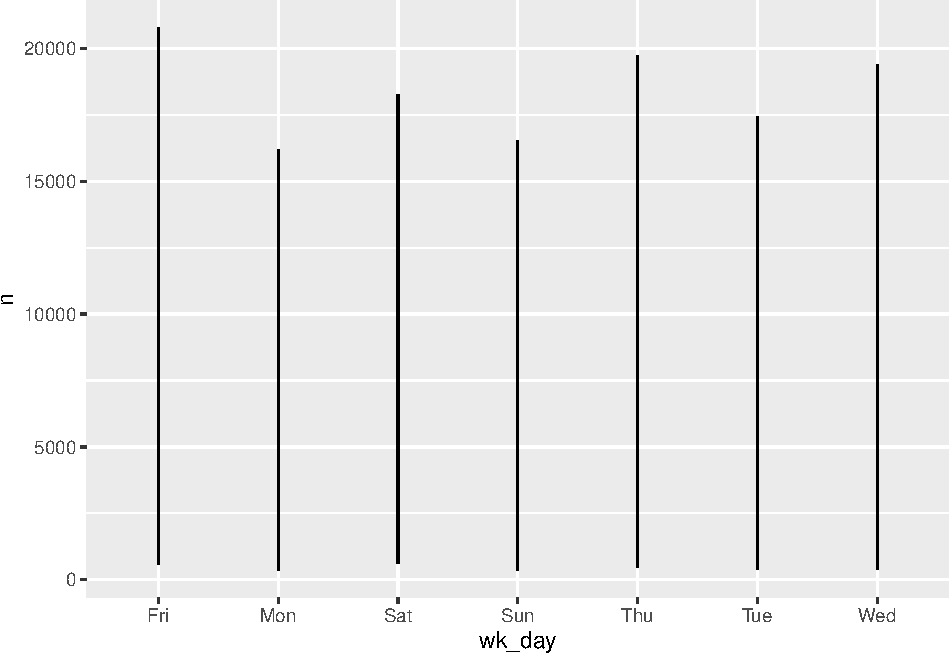
\includegraphics{R-data-viz_files/figure-latex/first-time-series-1.pdf}

Unfortunately, this does not work because we plotted data for all the
violations together. So what ggplot displays is the range of all values
for each year in a vertial line. We need to tell ggplot to draw a line
for each violation by modifying the aesthetic function to include
\texttt{group\ =\ violation}:

\begin{Shaded}
\begin{Highlighting}[]
\NormalTok{trafficstops }\OperatorTok\StringTok{ }
\StringTok{  }\KeywordTok{mutate}\NormalTok{(}\DataTypeTok{wk_day =} \KeywordTok{wday}\NormalTok{(stop_date, }\DataTypeTok{label =} \OtherTok{TRUE}\NormalTok{)) }\OperatorTok\StringTok{  }
\StringTok{  }\KeywordTok{group_by}\NormalTok{(wk_day, violation) }\OperatorTok
\StringTok{  }\NormalTok{tally }\OperatorTok\StringTok{ }
\StringTok{  }\KeywordTok{ggplot}\NormalTok{(}\KeywordTok{aes}\NormalTok{(}\DataTypeTok{x =}\NormalTok{ wk_day, }\DataTypeTok{y =}\NormalTok{ n, }\DataTypeTok{group =}\NormalTok{ violation)) }\OperatorTok{+}
\StringTok{     }\KeywordTok{geom_line}\NormalTok{()}
\end{Highlighting}
\end{Shaded}

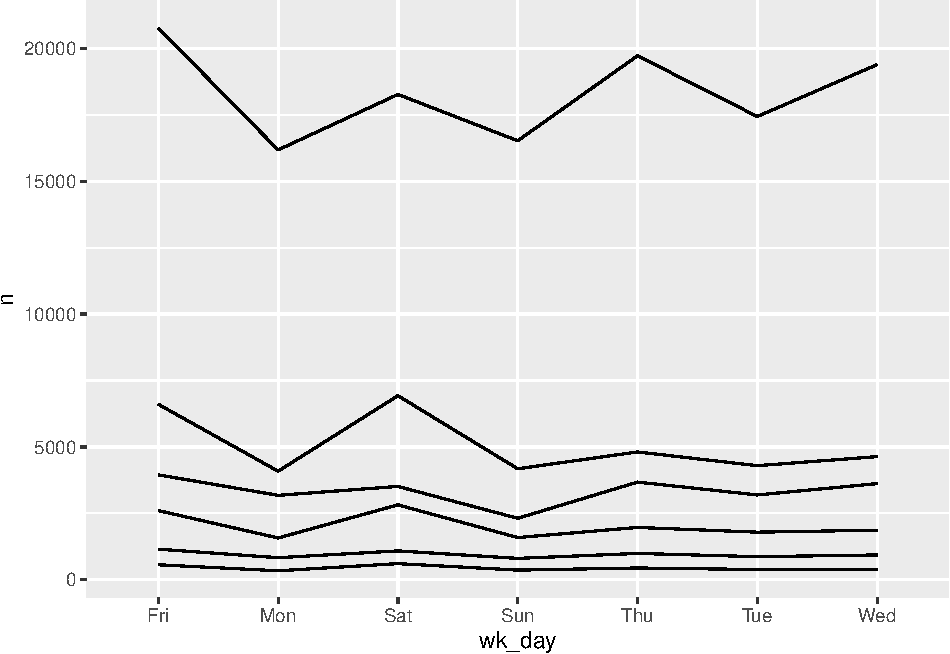
\includegraphics[width=0.7\linewidth]{R-data-viz_files/figure-latex/time-series-by-violation-1}

We will be able to distinguish violations in the plot if we add colors.
(Colors groups automatically if the variable is numeric).

\begin{Shaded}
\begin{Highlighting}[]
\NormalTok{trafficstops }\OperatorTok\StringTok{ }
\StringTok{  }\KeywordTok{mutate}\NormalTok{(}\DataTypeTok{wk_day =} \KeywordTok{wday}\NormalTok{(stop_date, }\DataTypeTok{label =} \OtherTok{TRUE}\NormalTok{)) }\OperatorTok\StringTok{  }
\StringTok{  }\KeywordTok{group_by}\NormalTok{(wk_day, violation) }\OperatorTok
\StringTok{  }\NormalTok{tally }\OperatorTok\StringTok{ }
\StringTok{  }\KeywordTok{ggplot}\NormalTok{(}\KeywordTok{aes}\NormalTok{(}\DataTypeTok{x =}\NormalTok{ wk_day, }\DataTypeTok{y =}\NormalTok{ n, }\DataTypeTok{group =}\NormalTok{ violation, }\DataTypeTok{color =}\NormalTok{ violation)) }\OperatorTok{+}
\StringTok{     }\KeywordTok{geom_line}\NormalTok{()}
\end{Highlighting}
\end{Shaded}

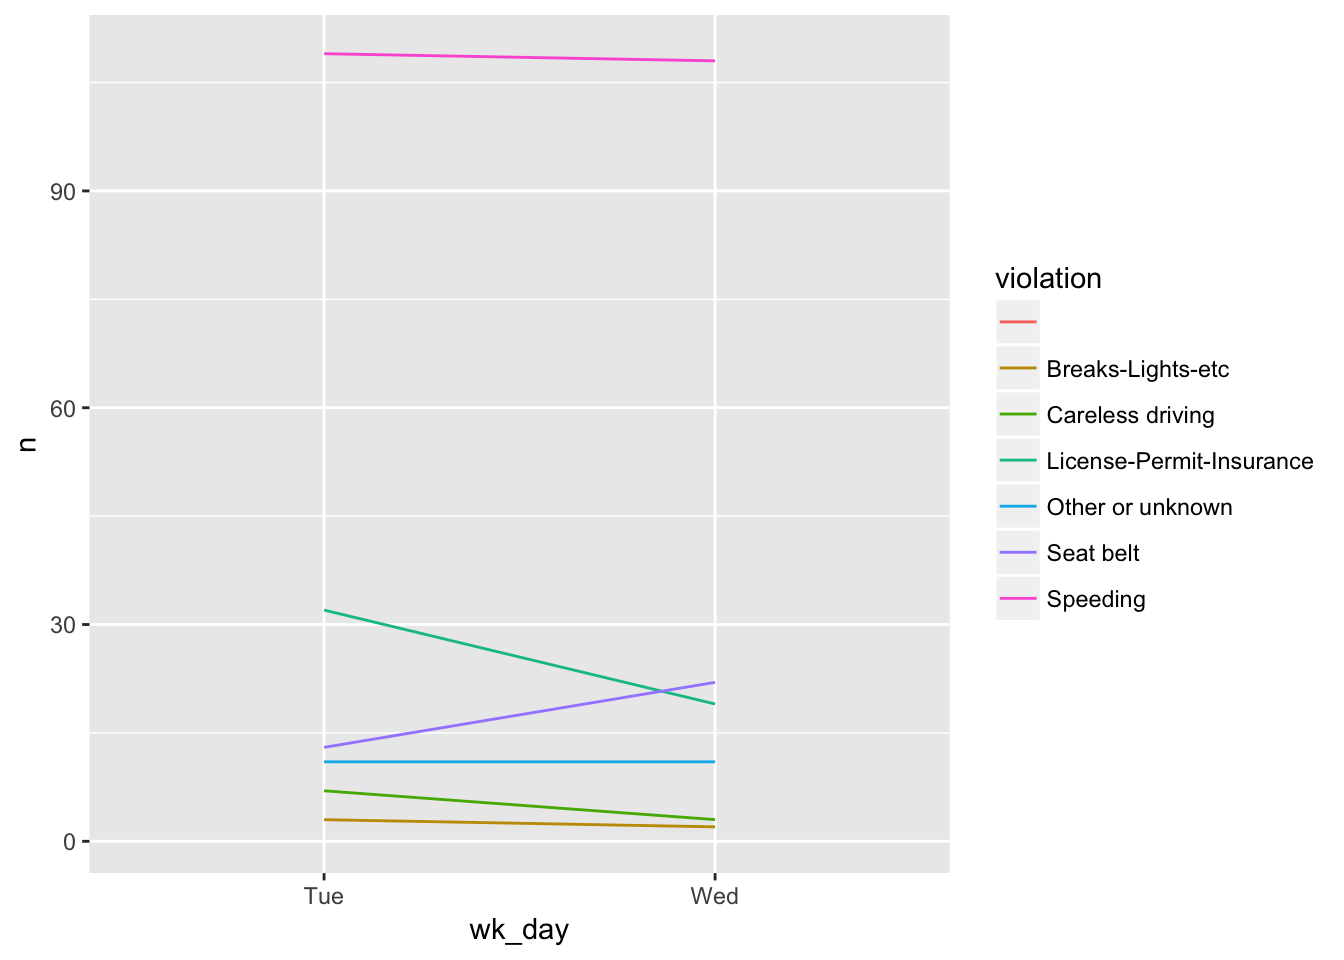
\includegraphics[width=0.7\linewidth]{R-data-viz_files/figure-latex/time-series-with-colors-1}

\section{Faceting}\label{faceting}

ggplot has a special technique called \emph{faceting} that allows to
split one plot into multiple plots based on a factor included in the
dataset. We will use it to make a time series plot for each violation:

\begin{Shaded}
\begin{Highlighting}[]
\NormalTok{trafficstops }\OperatorTok\StringTok{ }
\StringTok{  }\KeywordTok{mutate}\NormalTok{(}\DataTypeTok{wk_day =} \KeywordTok{wday}\NormalTok{(stop_date, }\DataTypeTok{label =} \OtherTok{TRUE}\NormalTok{)) }\OperatorTok\StringTok{  }
\StringTok{  }\KeywordTok{group_by}\NormalTok{(wk_day, violation) }\OperatorTok
\StringTok{  }\NormalTok{tally }\OperatorTok\StringTok{ }
\StringTok{  }\KeywordTok{ggplot}\NormalTok{(}\KeywordTok{aes}\NormalTok{(}\DataTypeTok{x =}\NormalTok{ wk_day, }\DataTypeTok{y =}\NormalTok{ n, }\DataTypeTok{group =}\NormalTok{ violation)) }\OperatorTok{+}
\StringTok{     }\KeywordTok{geom_line}\NormalTok{() }\OperatorTok{+}
\StringTok{     }\KeywordTok{facet_wrap}\NormalTok{(}\OperatorTok{~}\StringTok{ }\NormalTok{violation)}
\end{Highlighting}
\end{Shaded}

\begin{verbatim}
#> geom_path: Each group consists of only one observation. Do you need to
#> adjust the group aesthetic?
\end{verbatim}

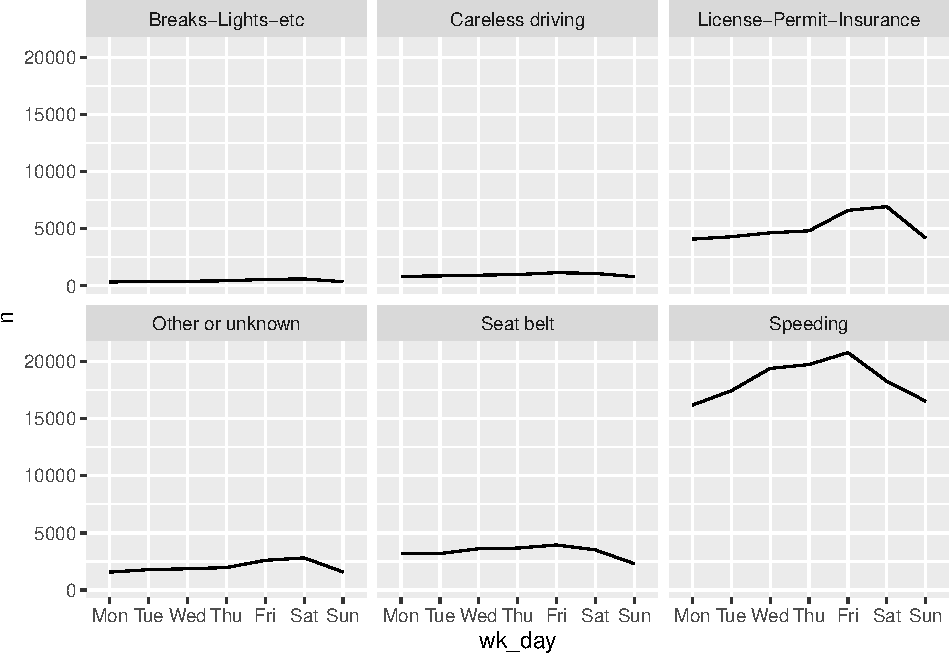
\includegraphics[width=0.7\linewidth]{R-data-viz_files/figure-latex/first-facet-1}

Now we would like to split the line in each plot by the race of the
driver. To do that we need to make counts in the data frame grouped by
\texttt{day}, \texttt{violation}, and \texttt{driver\_race}. We then
make the faceted plot by splitting further by race using \texttt{color}
and \texttt{group} (within a single plot):

\begin{Shaded}
\begin{Highlighting}[]
\NormalTok{trafficstops }\OperatorTok\StringTok{ }
\StringTok{  }\KeywordTok{mutate}\NormalTok{(}\DataTypeTok{wk_day =} \KeywordTok{wday}\NormalTok{(stop_date, }\DataTypeTok{label=}\OtherTok{TRUE}\NormalTok{)) }\OperatorTok\StringTok{ }
\StringTok{  }\KeywordTok{group_by}\NormalTok{(wk_day, violation, driver_race) }\OperatorTok
\StringTok{  }\NormalTok{tally }\OperatorTok\StringTok{ }
\StringTok{  }\KeywordTok{ggplot}\NormalTok{(}\KeywordTok{aes}\NormalTok{(}\DataTypeTok{x =}\NormalTok{ wk_day, }\DataTypeTok{y =}\NormalTok{ n, }\DataTypeTok{color =}\NormalTok{ driver_race, }\DataTypeTok{group =}\NormalTok{ driver_race)) }\OperatorTok{+}
\StringTok{  }\KeywordTok{geom_line}\NormalTok{() }\OperatorTok{+}\StringTok{ }
\StringTok{  }\KeywordTok{facet_wrap}\NormalTok{(}\OperatorTok{~}\StringTok{ }\NormalTok{violation)}
\end{Highlighting}
\end{Shaded}

\begin{verbatim}
#> geom_path: Each group consists of only one observation. Do you need to
#> adjust the group aesthetic?
\end{verbatim}

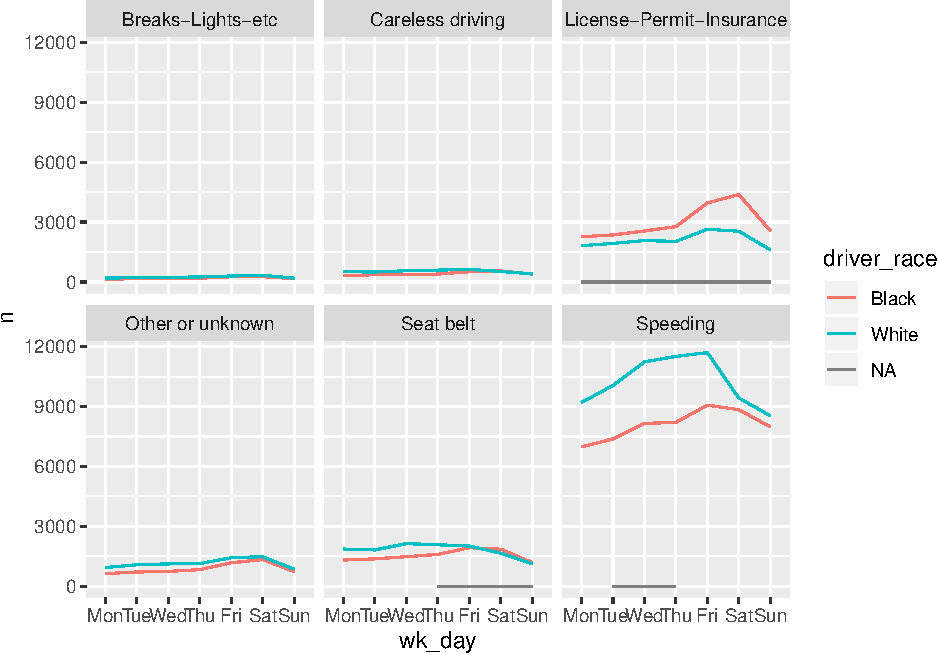
\includegraphics{R-data-viz_files/figure-latex/facet-by-violation-and-race-1.pdf}

Note that there is an alternative, the \texttt{facet\_grid} geometry,
which allows you to explicitly specify how you want your plots to be
arranged via formula notation
(\texttt{rows\ \textasciitilde{}\ columns}; a \texttt{.} can be used as
a placeholder that indicates only one row or column).

\begin{quote}
Challenge

Use what you just learned to create a plot that depicts how the average
age of each driver for the two recorded ethnicities changes through the
week. Hint: make sure you remove the records with driver\_age under 16.
How would you go about visualizing both lines and points on the plot?
How would you split your plot into one per each violation type?
\end{quote}

\section{\texorpdfstring{\textbf{\texttt{ggplot2}}
themes}{ggplot2 themes}}\label{ggplot2-themes}

\textbf{\texttt{ggplot2}} comes with several other themes which can be
useful to quickly change the look of your visualization, for example
\texttt{theme\_bw()} changes the plot background to white:

\begin{Shaded}
\begin{Highlighting}[]
\NormalTok{trafficstops }\OperatorTok\StringTok{ }
\StringTok{  }\KeywordTok{mutate}\NormalTok{(}\DataTypeTok{wk_day =} \KeywordTok{wday}\NormalTok{(stop_date, }\DataTypeTok{label=}\OtherTok{TRUE}\NormalTok{, }\DataTypeTok{abbr=}\OtherTok{TRUE}\NormalTok{)) }\OperatorTok\StringTok{ }
\StringTok{  }\KeywordTok{group_by}\NormalTok{(wk_day, violation, driver_race) }\OperatorTok
\StringTok{  }\NormalTok{tally }\OperatorTok\StringTok{ }
\StringTok{  }\KeywordTok{ggplot}\NormalTok{(}\KeywordTok{aes}\NormalTok{(}\DataTypeTok{x =}\NormalTok{ wk_day, }\DataTypeTok{y =}\NormalTok{ n, }\DataTypeTok{color =}\NormalTok{ driver_race, }\DataTypeTok{group =}\NormalTok{ driver_race)) }\OperatorTok{+}
\StringTok{  }\KeywordTok{geom_line}\NormalTok{() }\OperatorTok{+}\StringTok{ }
\StringTok{  }\KeywordTok{facet_wrap}\NormalTok{(}\OperatorTok{~}\StringTok{ }\NormalTok{violation) }\OperatorTok{+}
\StringTok{  }\KeywordTok{theme_bw}\NormalTok{()}
\end{Highlighting}
\end{Shaded}

\begin{verbatim}
#> geom_path: Each group consists of only one observation. Do you need to
#> adjust the group aesthetic?
\end{verbatim}

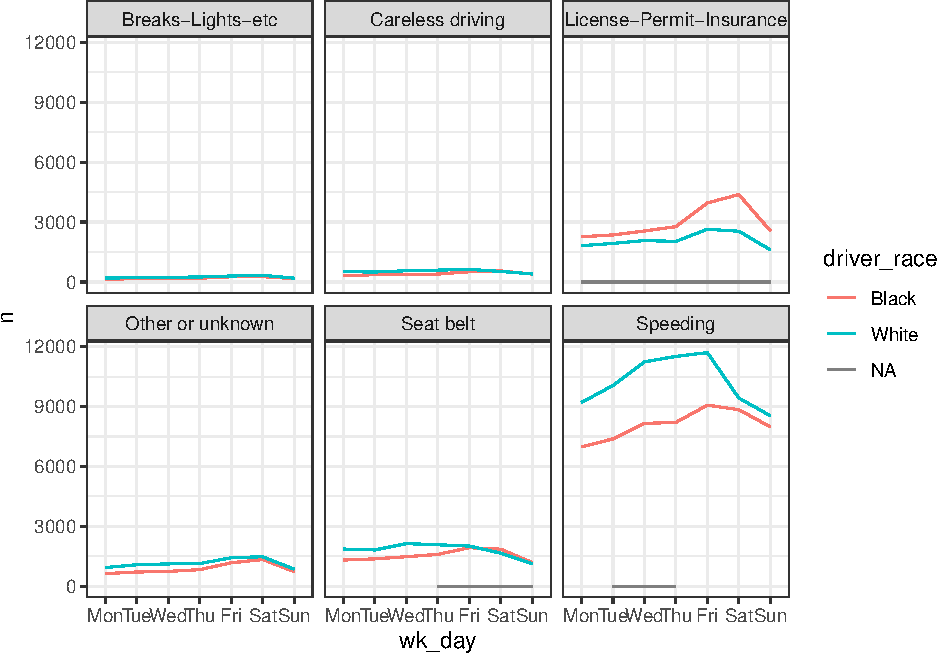
\includegraphics{R-data-viz_files/figure-latex/facet-theming-1.pdf}

The complete list of themes is available at
\url{http://docs.ggplot2.org/current/ggtheme.html}.
\texttt{theme\_minimal()} and \texttt{theme\_light()} are popular, and
\texttt{theme\_void()} can be useful as a starting point to create a new
hand-crafted theme.

The
\href{https://cran.r-project.org/web/packages/ggthemes/vignettes/ggthemes.html}{ggthemes}
package provides a wide variety of options (including an Excel 2003
theme). The
\href{https://www.ggplot2-exts.org}{\textbf{\texttt{ggplot2}} extensions
website} provides a list of packages that extend the capabilities of
\textbf{\texttt{ggplot2}}, including additional themes.

\section{Customization}\label{customization}

There are endless possibilities to customize your plot, particularly
when you are ready for publication or presentation. Let's look into just
a few examples. Before we do that we will assign our plot above to a
variable.

\begin{Shaded}
\begin{Highlighting}[]
\NormalTok{stops_facet_plot <-}\StringTok{ }\NormalTok{trafficstops }\OperatorTok\StringTok{ }
\StringTok{  }\KeywordTok{mutate}\NormalTok{(}\DataTypeTok{wk_day =} \KeywordTok{wday}\NormalTok{(stop_date, }\DataTypeTok{label=}\OtherTok{TRUE}\NormalTok{, }\DataTypeTok{abbr=}\OtherTok{TRUE}\NormalTok{)) }\OperatorTok\StringTok{ }
\StringTok{  }\KeywordTok{group_by}\NormalTok{(wk_day, violation, driver_race) }\OperatorTok
\StringTok{  }\NormalTok{tally }\OperatorTok\StringTok{ }
\StringTok{  }\KeywordTok{ggplot}\NormalTok{(}\KeywordTok{aes}\NormalTok{(}\DataTypeTok{x =}\NormalTok{ wk_day, }\DataTypeTok{y =}\NormalTok{ n, }\DataTypeTok{color =}\NormalTok{ driver_race, }\DataTypeTok{group =}\NormalTok{ driver_race)) }\OperatorTok{+}
\StringTok{  }\KeywordTok{geom_line}\NormalTok{() }\OperatorTok{+}\StringTok{ }
\StringTok{  }\KeywordTok{facet_wrap}\NormalTok{(}\OperatorTok{~}\StringTok{ }\NormalTok{violation)}
\end{Highlighting}
\end{Shaded}

Now, let's change names of axes to something more informative than
`wk\_day' and `n' and add a title to the figure:

\begin{Shaded}
\begin{Highlighting}[]
\NormalTok{stops_facet_plot }\OperatorTok{+}
\StringTok{  }\KeywordTok{labs}\NormalTok{(}\DataTypeTok{title =} \StringTok{'Observed violations per day of week'}\NormalTok{,}
         \DataTypeTok{x =} \StringTok{'Weekday of observation'}\NormalTok{,}
         \DataTypeTok{y =} \StringTok{'Number of violations'}\NormalTok{) }\OperatorTok{+}
\StringTok{  }\KeywordTok{theme_bw}\NormalTok{()}
\end{Highlighting}
\end{Shaded}

\begin{verbatim}
#> geom_path: Each group consists of only one observation. Do you need to
#> adjust the group aesthetic?
\end{verbatim}

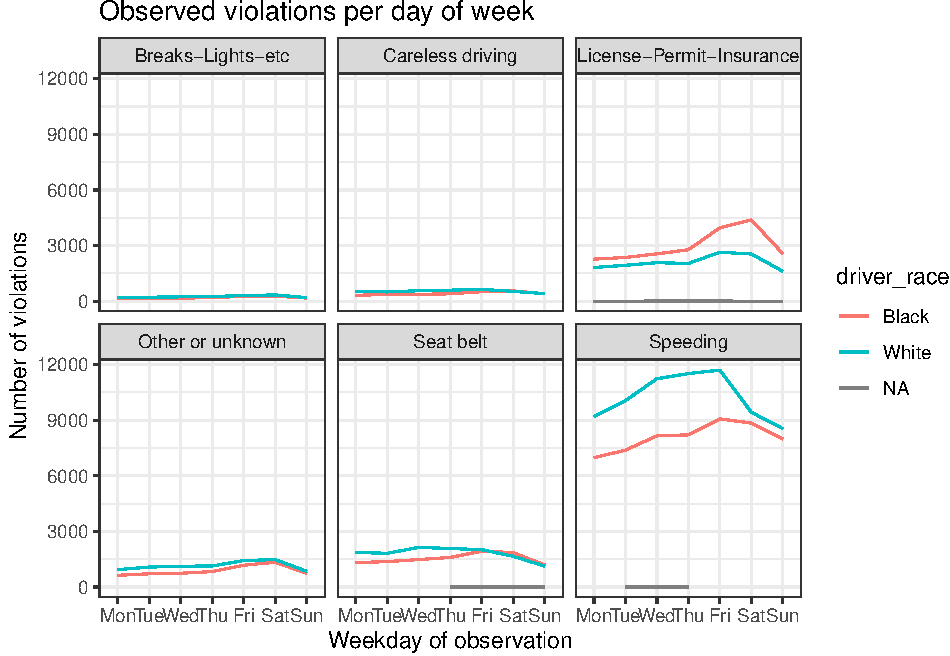
\includegraphics{R-data-viz_files/figure-latex/improved-labels-1.pdf}

The axes have more informative names, but their readability can be
improved by increasing the font size:

\begin{Shaded}
\begin{Highlighting}[]
\NormalTok{stops_facet_plot }\OperatorTok{+}
\StringTok{  }\KeywordTok{labs}\NormalTok{(}\DataTypeTok{title =} \StringTok{'Observed violations per day of week'}\NormalTok{,}
         \DataTypeTok{x =} \StringTok{'Weekday of observation'}\NormalTok{,}
         \DataTypeTok{y =} \StringTok{'Number of violations'}\NormalTok{) }\OperatorTok{+}
\StringTok{  }\KeywordTok{theme_bw}\NormalTok{() }\OperatorTok{+}\StringTok{ }
\StringTok{  }\KeywordTok{theme}\NormalTok{(}\DataTypeTok{text =} \KeywordTok{element_text}\NormalTok{(}\DataTypeTok{size=}\DecValTok{16}\NormalTok{))}
\end{Highlighting}
\end{Shaded}

\begin{verbatim}
#> geom_path: Each group consists of only one observation. Do you need to
#> adjust the group aesthetic?
\end{verbatim}

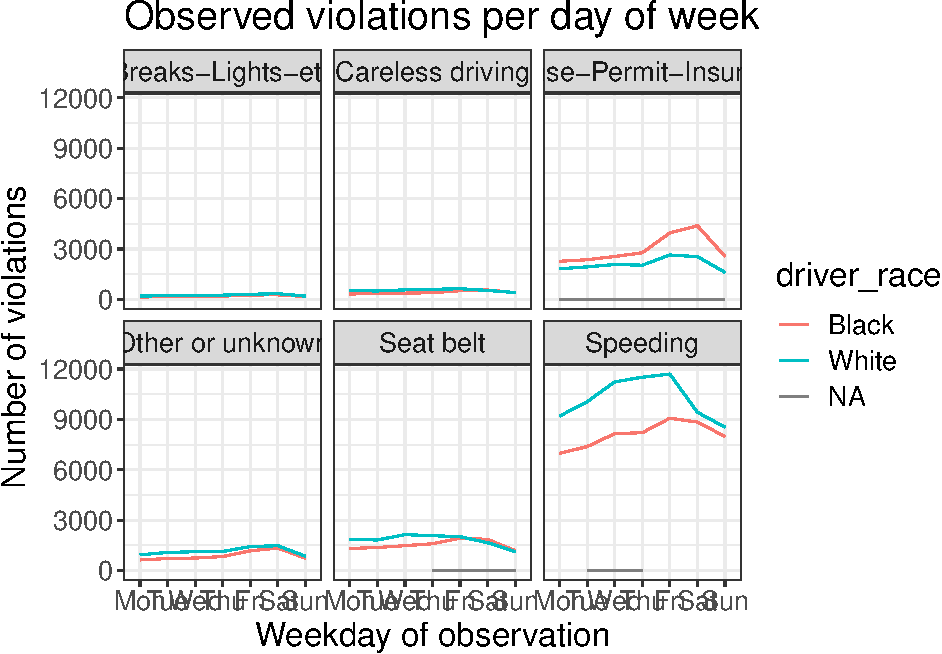
\includegraphics{R-data-viz_files/figure-latex/improved-font-size-1.pdf}

After our manipulations, you may notice that the values on the x-axis
are still not properly readable. Let's change the orientation of the
labels and adjust them vertically and horizontally so they don't
overlap. You can use a 90 degree angle, or experiment to find the
appropriate angle for diagonally oriented labels:

\begin{Shaded}
\begin{Highlighting}[]
\NormalTok{stops_facet_plot }\OperatorTok{+}
\StringTok{  }\KeywordTok{labs}\NormalTok{(}\DataTypeTok{title =} \StringTok{'Observed violations per day of week'}\NormalTok{,}
         \DataTypeTok{x =} \StringTok{'Weekday of observation'}\NormalTok{,}
         \DataTypeTok{y =} \StringTok{'Number of violations'}\NormalTok{) }\OperatorTok{+}
\StringTok{  }\KeywordTok{theme_bw}\NormalTok{() }\OperatorTok{+}\StringTok{ }
\StringTok{  }\KeywordTok{theme}\NormalTok{(}\DataTypeTok{axis.text.x =} \KeywordTok{element_text}\NormalTok{(}\DataTypeTok{colour=}\StringTok{"grey40"}\NormalTok{, }\DataTypeTok{size=}\DecValTok{12}\NormalTok{, }\DataTypeTok{angle=}\DecValTok{90}\NormalTok{, }\DataTypeTok{hjust=}\NormalTok{.}\DecValTok{5}\NormalTok{, }\DataTypeTok{vjust=}\NormalTok{.}\DecValTok{5}\NormalTok{),}
        \DataTypeTok{axis.text.y =} \KeywordTok{element_text}\NormalTok{(}\DataTypeTok{colour=}\StringTok{"grey40"}\NormalTok{, }\DataTypeTok{size=}\DecValTok{12}\NormalTok{),}
        \DataTypeTok{strip.text =} \KeywordTok{element_text}\NormalTok{(}\DataTypeTok{size=}\DecValTok{14}\NormalTok{),}
        \DataTypeTok{text =} \KeywordTok{element_text}\NormalTok{(}\DataTypeTok{size=}\DecValTok{16}\NormalTok{))}
\end{Highlighting}
\end{Shaded}

\begin{verbatim}
#> geom_path: Each group consists of only one observation. Do you need to
#> adjust the group aesthetic?
\end{verbatim}

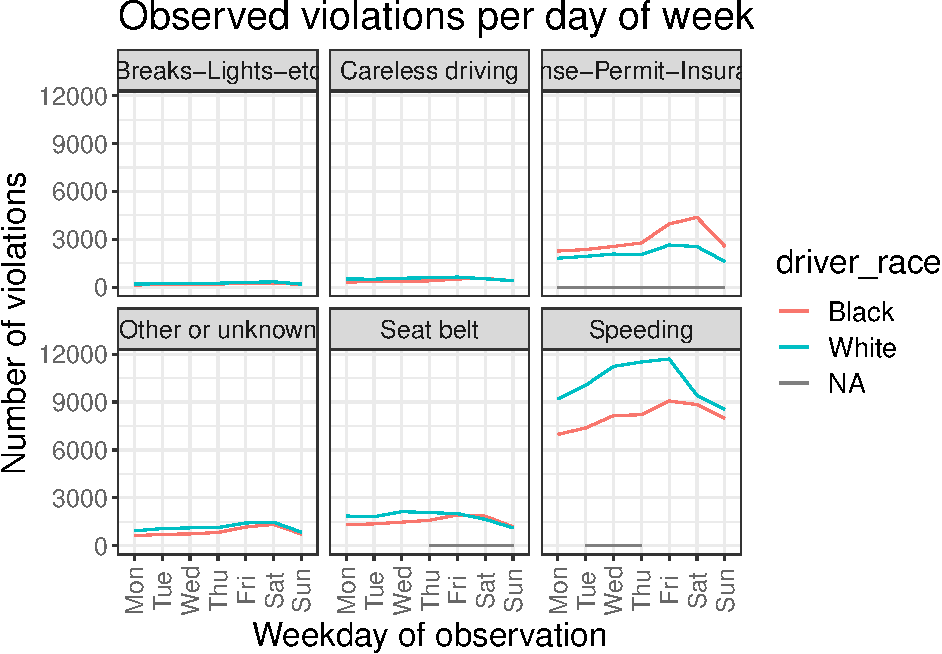
\includegraphics{R-data-viz_files/figure-latex/tilted-xlabels-1.pdf}

If you like the changes you created better than the default theme, you
can save them as an object to be able to easily apply them to other
plots you may create:

\begin{Shaded}
\begin{Highlighting}[]
\NormalTok{grey_theme <-}\StringTok{ }\KeywordTok{theme}\NormalTok{(}\DataTypeTok{axis.text.x =} \KeywordTok{element_text}\NormalTok{(}\DataTypeTok{colour=}\StringTok{"grey40"}\NormalTok{, }\DataTypeTok{size=}\DecValTok{12}\NormalTok{, }\DataTypeTok{angle=}\DecValTok{90}\NormalTok{, }\DataTypeTok{hjust=}\NormalTok{.}\DecValTok{5}\NormalTok{, }\DataTypeTok{vjust=}\NormalTok{.}\DecValTok{5}\NormalTok{),}
                   \DataTypeTok{axis.text.y =} \KeywordTok{element_text}\NormalTok{(}\DataTypeTok{colour=}\StringTok{"grey40"}\NormalTok{, }\DataTypeTok{size=}\DecValTok{12}\NormalTok{), }\DataTypeTok{text=}\KeywordTok{element_text}\NormalTok{(}\DataTypeTok{size=}\DecValTok{16}\NormalTok{))}

\KeywordTok{ggplot}\NormalTok{(}\DataTypeTok{data =}\NormalTok{ Chickasaw_stops, }\KeywordTok{aes}\NormalTok{(}\DataTypeTok{x =}\NormalTok{ violation, }\DataTypeTok{y =}\NormalTok{ driver_age)) }\OperatorTok{+}
\StringTok{  }\KeywordTok{geom_boxplot}\NormalTok{() }\OperatorTok{+}\StringTok{ }
\StringTok{  }\NormalTok{grey_theme}
\end{Highlighting}
\end{Shaded}

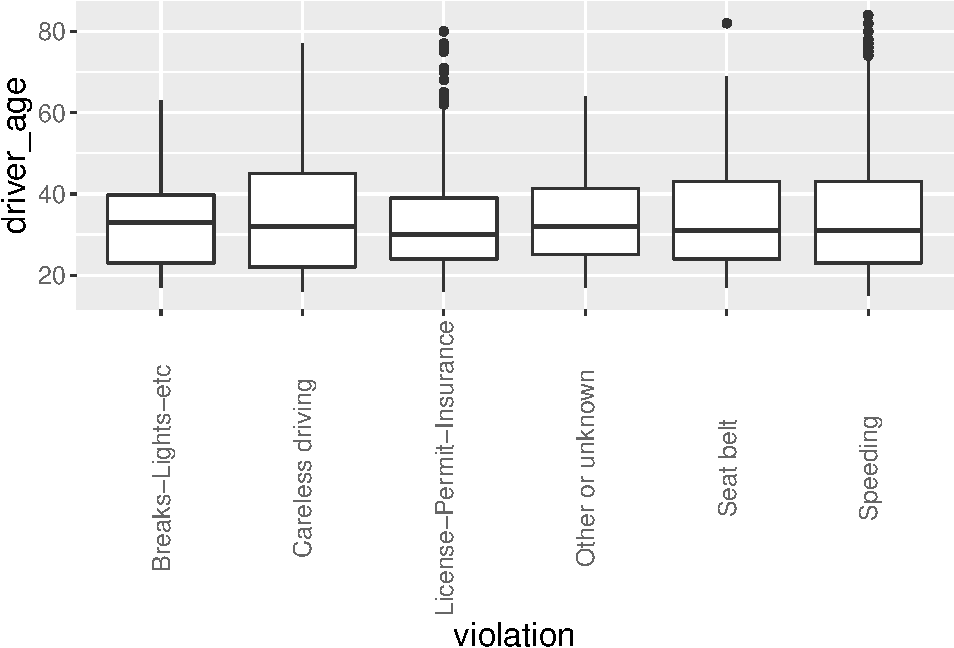
\includegraphics{R-data-viz_files/figure-latex/save-reapply-theme-1.pdf}

Note that it is also possible to change the fonts of your plots. If you
are on Windows, you may have to install the
\href{https://github.com/wch/extrafont}{\textbf{extrafont} package}, and
follow the instructions included in the README for this package.

\begin{quote}
Challenge

With all of this information in hand, please take another five minutes
to either improve one of the plots generated in this exercise or create
a beautiful graph of your own. Use the RStudio
\href{https://www.rstudio.com/wp-content/uploads/2016/11/ggplot2-cheatsheet-2.1.pdf}{\textbf{\texttt{ggplot2}}
cheat sheet} for inspiration.
\end{quote}

\begin{quote}
Here are some ideas:
\end{quote}

\begin{quote}
\begin{itemize}
\tightlist
\item
  See if you can change the thickness of the lines.
\item
  Can you find a way to change the name of the legend? What about its
  labels?
\item
  Try using a different color palette (see
  \url{http://www.cookbook-r.com/Graphs/Colors_(ggplot2)/}).
\end{itemize}
\end{quote}

After creating your plot, you can save it out to a file in your prefered
format. You can change the dimension (and resolution) of your plot by
adjusting the appropriate arguments (\texttt{width}, \texttt{height} and
\texttt{dpi}):

\begin{Shaded}
\begin{Highlighting}[]
\NormalTok{my_plot <-}\StringTok{ }\NormalTok{stops_facet_plot }\OperatorTok{+}
\StringTok{  }\KeywordTok{labs}\NormalTok{(}\DataTypeTok{title =} \StringTok{'Observed violations per day of week'}\NormalTok{,}
         \DataTypeTok{x =} \StringTok{'Weekday of observation'}\NormalTok{,}
         \DataTypeTok{y =} \StringTok{'Number of violations'}\NormalTok{) }\OperatorTok{+}
\StringTok{  }\KeywordTok{theme_bw}\NormalTok{() }\OperatorTok{+}\StringTok{ }
\StringTok{  }\KeywordTok{theme}\NormalTok{(}\DataTypeTok{axis.text.x =} \KeywordTok{element_text}\NormalTok{(}\DataTypeTok{colour=}\StringTok{"grey40"}\NormalTok{, }\DataTypeTok{size=}\DecValTok{12}\NormalTok{, }\DataTypeTok{angle=}\DecValTok{90}\NormalTok{, }\DataTypeTok{hjust=}\NormalTok{.}\DecValTok{5}\NormalTok{, }\DataTypeTok{vjust=}\NormalTok{.}\DecValTok{5}\NormalTok{),}
        \DataTypeTok{axis.text.y =} \KeywordTok{element_text}\NormalTok{(}\DataTypeTok{colour=}\StringTok{"grey40"}\NormalTok{, }\DataTypeTok{size=}\DecValTok{12}\NormalTok{),}
        \DataTypeTok{strip.text =} \KeywordTok{element_text}\NormalTok{(}\DataTypeTok{size=}\DecValTok{14}\NormalTok{),}
        \DataTypeTok{text =} \KeywordTok{element_text}\NormalTok{(}\DataTypeTok{size=}\DecValTok{16}\NormalTok{))}

\KeywordTok{ggsave}\NormalTok{(}\StringTok{"name_of_file.png"}\NormalTok{, my_plot, }\DataTypeTok{width=}\DecValTok{15}\NormalTok{, }\DataTypeTok{height=}\DecValTok{10}\NormalTok{)}
\end{Highlighting}
\end{Shaded}

Note: The parameters \texttt{width} and \texttt{height} also determine
the font size in the saved plot.

\chapter{\texorpdfstring{Alternatives: R base \texttt{plot} and
\texttt{lattice}
graphs}{Alternatives: R base plot and lattice graphs}}\label{baseplot}

\begin{quote}
Learning Objectives

\begin{itemize}
\tightlist
\item
  Make a plot with base plot package
\item
  Make a plot with other base plot commands
\item
  Make a simple plot with R lattice package
\item
  Explain the difference between this and ggplot approach - evaluate
  pros and cons
\end{itemize}
\end{quote}

\begin{center}\rule{0.5\linewidth}{\linethickness}\end{center}

\section{\texorpdfstring{R base \texttt{plot}
commands}{R base plot commands}}\label{r-base-plot-commands}

We will use a simple dataset that comes with the base R install.
\textbf{USE DIFFERENT DATA}

\begin{Shaded}
\begin{Highlighting}[]
\KeywordTok{head}\NormalTok{(cars)}
\end{Highlighting}
\end{Shaded}

\begin{verbatim}
#>   speed dist
#> 1     4    2
#> 2     4   10
#> 3     7    4
#> 4     7   22
#> 5     8   16
#> 6     9   10
\end{verbatim}

R base comes wiht a simple plot command that can be applied to the data
like that:

\begin{Shaded}
\begin{Highlighting}[]
\KeywordTok{plot}\NormalTok{(cars)}
\end{Highlighting}
\end{Shaded}

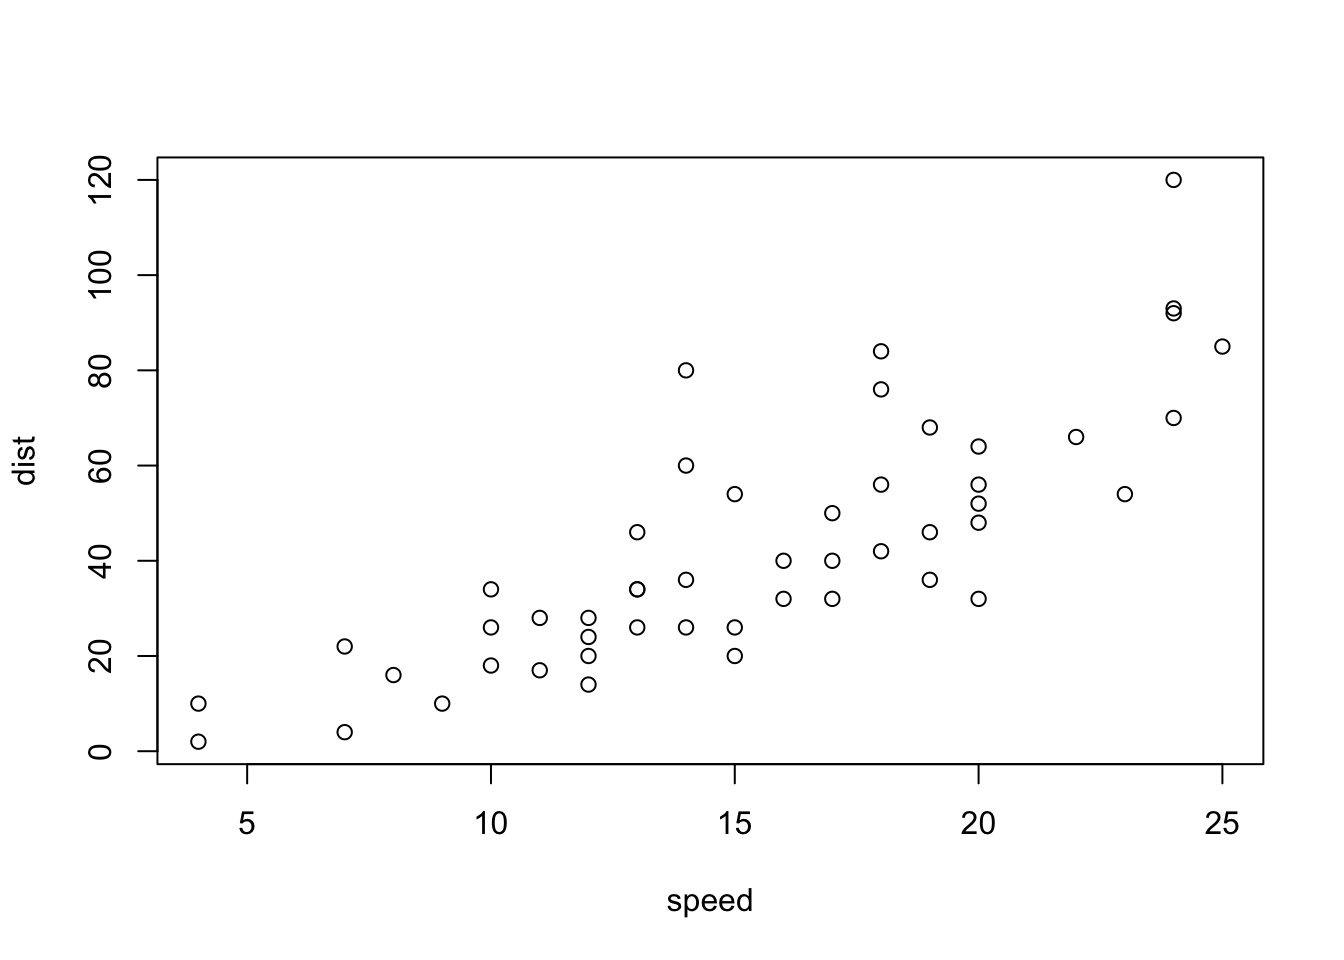
\includegraphics{R-data-viz_files/figure-latex/plot-cars-1.pdf}

Other things one can do with plot. Walk through arguments. How to do
multiple plots.

\url{https://www.stat.auckland.ac.nz/~paul/RGraphics/chapter1.pdf} and
code:
\url{https://www.stat.auckland.ac.nz/~paul/RGraphics/chapter1.html}

\begin{quote}
Challenge: make a plot
\end{quote}

\begin{quote}
Challenge: how would you do this with ggplot?
\end{quote}

Lastly, there is \texttt{ggplot}. Which works like this:

Other base package plot commands: histogram, boxplot, stripchart,
barplot, mosaicplot.. dotchart

\url{http://www.cyclismo.org/tutorial/R/plotting.html} and
\url{http://www.cyclismo.org/tutorial/R/intermediatePlotting.html}

\url{https://www.harding.edu/fmccown/r/}

\url{http://courses.atlas.illinois.edu/spring2017/STAT/STAT200/RProgramming/Plotting.html}

\begin{quote}
Challenge: use some of these commands
\end{quote}

\section{\texorpdfstring{\texttt{lattice}
package}{lattice package}}\label{lattice-package}

Lattice is another major graphic package in R. {[}\ldots{} more about it
here\ldots{}{]} It works like this:

\begin{Shaded}
\begin{Highlighting}[]
\KeywordTok{xyplot}\NormalTok{(dist }\OperatorTok{~}\StringTok{ }\NormalTok{speed, cars)}
\end{Highlighting}
\end{Shaded}

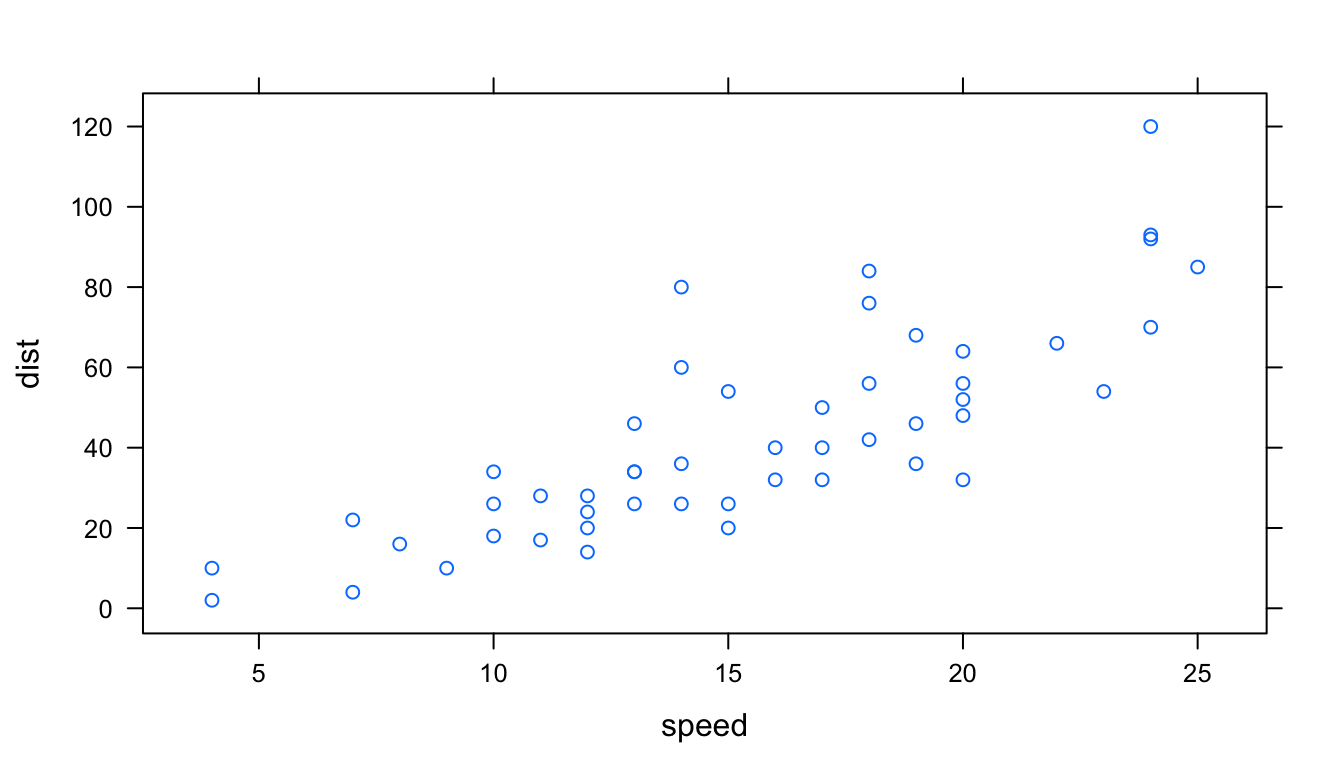
\includegraphics{R-data-viz_files/figure-latex/lattice-cars-1.pdf}

Iris data example (again, other data??) :

\begin{Shaded}
\begin{Highlighting}[]
\KeywordTok{head}\NormalTok{(iris)}
\end{Highlighting}
\end{Shaded}

\begin{verbatim}
#>   Sepal.Length Sepal.Width Petal.Length Petal.Width Species
#> 1          5.1         3.5          1.4         0.2  setosa
#> 2          4.9         3.0          1.4         0.2  setosa
#> 3          4.7         3.2          1.3         0.2  setosa
#> 4          4.6         3.1          1.5         0.2  setosa
#> 5          5.0         3.6          1.4         0.2  setosa
#> 6          5.4         3.9          1.7         0.4  setosa
\end{verbatim}

Contains 50 samples from 3 species with 4 measurements: length and width
of petals and length and width of sepals.

\begin{figure}
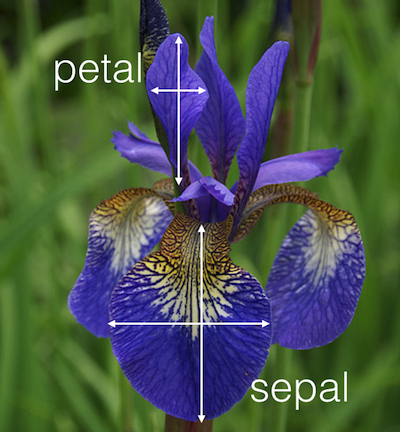
\includegraphics[width=0.3\linewidth]{img/iris_petal_sepal} \caption{Iris Petal and Sepal (Source: kaggle.com)}\label{fig:iris-photo}
\end{figure}

With \texttt{lattice}

\begin{Shaded}
\begin{Highlighting}[]
\KeywordTok{xyplot}\NormalTok{(Petal.Length}\OperatorTok{~}\NormalTok{Petal.Width, }\DataTypeTok{data =}\NormalTok{ iris, }\DataTypeTok{groups=}\NormalTok{Species, }
  \DataTypeTok{panel =}\NormalTok{ panel.superpose, }\DataTypeTok{type =} \KeywordTok{c}\NormalTok{(}\StringTok{"p"}\NormalTok{, }\StringTok{"smooth"}\NormalTok{), }\DataTypeTok{span=}\NormalTok{.}\DecValTok{75}\NormalTok{,}
  \DataTypeTok{col.line =} \KeywordTok{trellis.par.get}\NormalTok{(}\StringTok{"strip.background"}\NormalTok{)}\OperatorTok{$}\NormalTok{col,}
  \DataTypeTok{col.symbol =} \KeywordTok{trellis.par.get}\NormalTok{(}\StringTok{"strip.shingle"}\NormalTok{)}\OperatorTok{$}\NormalTok{col,}
  \DataTypeTok{key =} \KeywordTok{list}\NormalTok{(}\DataTypeTok{title=}\StringTok{"Iris Data"}\NormalTok{, }\DataTypeTok{x=}\NormalTok{.}\DecValTok{15}\NormalTok{, }\DataTypeTok{y=}\NormalTok{.}\DecValTok{85}\NormalTok{, }\DataTypeTok{corner=}\KeywordTok{c}\NormalTok{(}\DecValTok{0}\NormalTok{,}\DecValTok{1}\NormalTok{), }\DataTypeTok{border=}\OtherTok{TRUE}\NormalTok{,}
        \DataTypeTok{points =} \KeywordTok{list}\NormalTok{(}\DataTypeTok{col=}\KeywordTok{trellis.par.get}\NormalTok{(}\StringTok{"strip.shingle"}\NormalTok{)}\OperatorTok{$}\NormalTok{col[}\DecValTok{1}\OperatorTok{:}\DecValTok{3}\NormalTok{],}
                 \DataTypeTok{pch =} \KeywordTok{trellis.par.get}\NormalTok{(}\StringTok{"superpose.symbol"}\NormalTok{)}\OperatorTok{$}\NormalTok{pch[}\DecValTok{1}\OperatorTok{:}\DecValTok{3}\NormalTok{],}
                 \DataTypeTok{cex =} \KeywordTok{trellis.par.get}\NormalTok{(}\StringTok{"superpose.symbol"}\NormalTok{)}\OperatorTok{$}\NormalTok{cex[}\DecValTok{1}\OperatorTok{:}\DecValTok{3}\NormalTok{]),}
                 \DataTypeTok{text =} \KeywordTok{list}\NormalTok{(}\KeywordTok{levels}\NormalTok{(iris}\OperatorTok{$}\NormalTok{Species))))}
\end{Highlighting}
\end{Shaded}

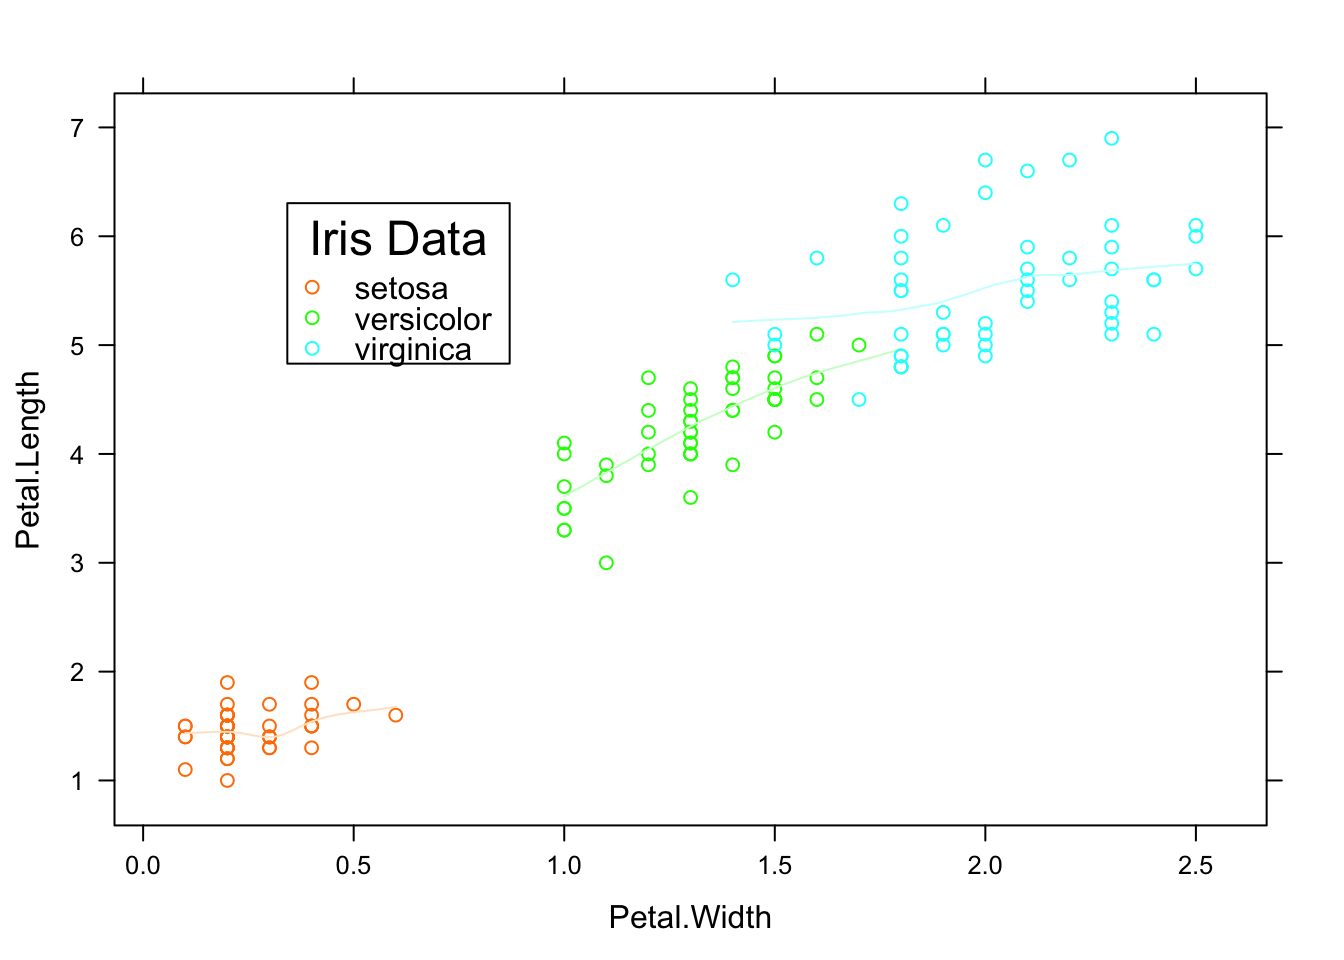
\includegraphics{R-data-viz_files/figure-latex/lattice-iris-1.pdf}

The same with ggplot:

\begin{Shaded}
\begin{Highlighting}[]
\KeywordTok{ggplot}\NormalTok{(}\DataTypeTok{data=}\NormalTok{iris, }\KeywordTok{aes}\NormalTok{(}\DataTypeTok{x=}\NormalTok{Petal.Width, }\DataTypeTok{y=}\NormalTok{Petal.Length, }\DataTypeTok{color=}\NormalTok{Species)) }\OperatorTok{+}
\StringTok{  }\KeywordTok{geom_point}\NormalTok{() }\OperatorTok{+}
\StringTok{  }\KeywordTok{stat_smooth}\NormalTok{(}\KeywordTok{aes}\NormalTok{(}\KeywordTok{jitter}\NormalTok{(Petal.Width), }\KeywordTok{jitter}\NormalTok{(Petal.Length)), }\DataTypeTok{size=}\NormalTok{.}\DecValTok{2}\NormalTok{, }\DataTypeTok{se=}\NormalTok{F) }\OperatorTok{+}
\StringTok{  }\KeywordTok{theme_classic}\NormalTok{()}
\end{Highlighting}
\end{Shaded}

\begin{verbatim}
#> `geom_smooth()` using method = 'loess'
\end{verbatim}

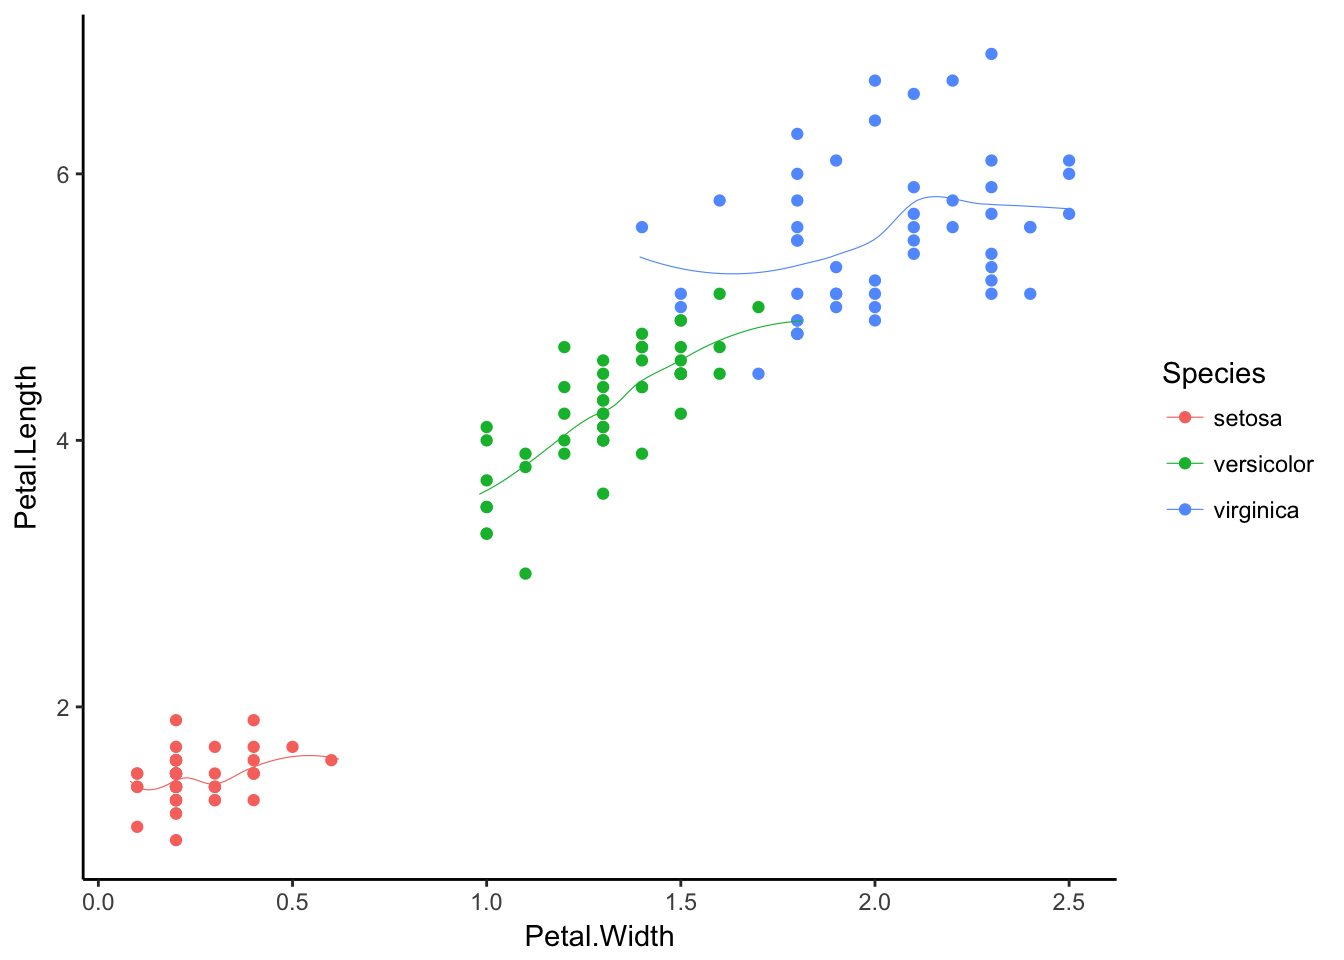
\includegraphics{R-data-viz_files/figure-latex/ggplot-iris-1.pdf}

pros - cons?

More about \texttt{lattice}:

\url{https://www.stat.auckland.ac.nz/~paul/RGraphics/chapter4.pdf} R
code:
\url{https://www.stat.auckland.ac.nz/~paul/RGraphics/chapter4.html}

\chapter{Domain specific graphs}\label{domains}

\begin{quote}
Learning Objectives

\begin{itemize}
\tightlist
\item
  Be aware of specialized graph packages and know where to look for them
\item
  Understand the basic structure of iheatmapr, tmap, and visNetwork
  examples
\item
  Modify parameters of provided graph examples
\end{itemize}
\end{quote}

\begin{center}\rule{0.5\linewidth}{\linethickness}\end{center}

\texttt{ggplot} can get you a long way, but if you need to do a
particular, more complex graph it is worth checking if there might be an
R package for that. Typically it would do one type of visualization and
do that really well. Below are a few examples.

\section{\texorpdfstring{Heatmaps (e.g.
\textbf{\texttt{iheatmapr}})}{Heatmaps (e.g. iheatmapr)}}\label{heatmaps-e.g.-iheatmapr}

\begin{Shaded}
\begin{Highlighting}[]
\KeywordTok{library}\NormalTok{(iheatmapr)}
\KeywordTok{data}\NormalTok{(measles, }\DataTypeTok{package =} \StringTok{"iheatmapr"}\NormalTok{)}

\KeywordTok{main_heatmap}\NormalTok{(measles, }\DataTypeTok{name =} \StringTok{"Measles<br>Cases"}\NormalTok{, }\DataTypeTok{x_categorical =} \OtherTok{FALSE}\NormalTok{,}
             \DataTypeTok{layout =} \KeywordTok{list}\NormalTok{(}\DataTypeTok{font =} \KeywordTok{list}\NormalTok{(}\DataTypeTok{size =} \DecValTok{8}\NormalTok{))) }\OperatorTok
\StringTok{  }\KeywordTok{add_col_groups}\NormalTok{(}\KeywordTok{ifelse}\NormalTok{(}\DecValTok{1930}\OperatorTok{:}\DecValTok{2001} \OperatorTok{<}\StringTok{ }\DecValTok{1961}\NormalTok{,}\StringTok{"No"}\NormalTok{,}\StringTok{"Yes"}\NormalTok{),}
                  \DataTypeTok{side =} \StringTok{"bottom"}\NormalTok{, }\DataTypeTok{name =} \StringTok{"Vaccine<br>Introduced?"}\NormalTok{,}
                  \DataTypeTok{title =} \StringTok{"Vaccine?"}\NormalTok{,}
                  \DataTypeTok{colors =} \KeywordTok{c}\NormalTok{(}\StringTok{"lightgray"}\NormalTok{,}\StringTok{"blue"}\NormalTok{)) }\OperatorTok
\StringTok{  }\KeywordTok{add_col_labels}\NormalTok{(}\DataTypeTok{ticktext =} \KeywordTok{seq}\NormalTok{(}\DecValTok{1930}\NormalTok{,}\DecValTok{2000}\NormalTok{,}\DecValTok{10}\NormalTok{),}\DataTypeTok{font =} \KeywordTok{list}\NormalTok{(}\DataTypeTok{size =} \DecValTok{8}\NormalTok{)) }\OperatorTok
\StringTok{  }\KeywordTok{add_row_labels}\NormalTok{(}\DataTypeTok{size =} \FloatTok{0.3}\NormalTok{,}\DataTypeTok{font =} \KeywordTok{list}\NormalTok{(}\DataTypeTok{size =} \DecValTok{6}\NormalTok{)) }\OperatorTok\StringTok{ }
\StringTok{  }\KeywordTok{add_col_summary}\NormalTok{(}\DataTypeTok{layout =} \KeywordTok{list}\NormalTok{(}\DataTypeTok{title =} \StringTok{"Average<br>across<br>states"}\NormalTok{),}
                  \DataTypeTok{yname =} \StringTok{"summary"}\NormalTok{)  }\OperatorTok\StringTok{                 }
\StringTok{  }\KeywordTok{add_col_title}\NormalTok{(}\StringTok{"Measles Cases from 1930 to 2001"}\NormalTok{, }\DataTypeTok{side=} \StringTok{"top"}\NormalTok{) }\OperatorTok
\StringTok{  }\KeywordTok{add_row_summary}\NormalTok{(}\DataTypeTok{groups =} \OtherTok{TRUE}\NormalTok{, }
                  \DataTypeTok{type =} \StringTok{"bar"}\NormalTok{,}
                  \DataTypeTok{layout =} \KeywordTok{list}\NormalTok{(}\DataTypeTok{title =} \StringTok{"Average<br>per<br>year"}\NormalTok{,}
                                \DataTypeTok{font =} \KeywordTok{list}\NormalTok{(}\DataTypeTok{size =} \DecValTok{8}\NormalTok{)))}
\end{Highlighting}
\end{Shaded}

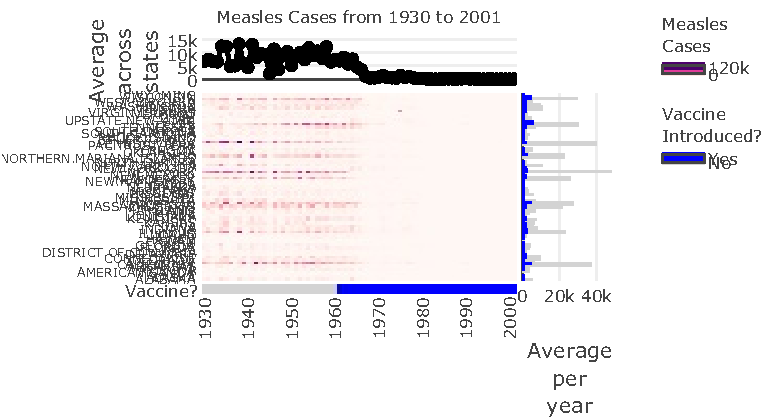
\includegraphics{R-data-viz_files/figure-latex/heatmap-demo-1.pdf}

\section{\texorpdfstring{Networks (e.g.
\textbf{\texttt{visNetwork}})}{Networks (e.g. visNetwork)}}\label{networks-e.g.-visnetwork}

\begin{Shaded}
\begin{Highlighting}[]
\KeywordTok{library}\NormalTok{(}\StringTok{'visNetwork'}\NormalTok{) }
\NormalTok{nodes <-}\StringTok{ }\KeywordTok{read.csv}\NormalTok{(}\StringTok{"demo-data/network/Dataset1-Media-Example-NODES.csv"}\NormalTok{, }\DataTypeTok{header=}\NormalTok{T, }\DataTypeTok{as.is=}\NormalTok{T)}
\NormalTok{links <-}\StringTok{ }\KeywordTok{read.csv}\NormalTok{(}\StringTok{"demo-data/network/Dataset1-Media-Example-EDGES.csv"}\NormalTok{, }\DataTypeTok{header=}\NormalTok{T, }\DataTypeTok{as.is=}\NormalTok{T)}
\NormalTok{nodes}\OperatorTok{$}\NormalTok{shape <-}\StringTok{ "dot"}  
\NormalTok{nodes}\OperatorTok{$}\NormalTok{shadow <-}\StringTok{ }\OtherTok{TRUE} \CommentTok{# Nodes will drop shadow}
\NormalTok{nodes}\OperatorTok{$}\NormalTok{title <-}\StringTok{ }\NormalTok{nodes}\OperatorTok{$}\NormalTok{media }\CommentTok{# Text on click}
\NormalTok{nodes}\OperatorTok{$}\NormalTok{label <-}\StringTok{ }\NormalTok{nodes}\OperatorTok{$}\NormalTok{type.label }\CommentTok{# Node label}
\NormalTok{nodes}\OperatorTok{$}\NormalTok{size <-}\StringTok{ }\NormalTok{nodes}\OperatorTok{$}\NormalTok{audience.size }\CommentTok{# Node size}
\NormalTok{nodes}\OperatorTok{$}\NormalTok{borderWidth <-}\StringTok{ }\DecValTok{2} \CommentTok{# Node border width}

\NormalTok{nodes}\OperatorTok{$}\NormalTok{color.background <-}\StringTok{ }\KeywordTok{c}\NormalTok{(}\StringTok{"slategrey"}\NormalTok{, }\StringTok{"tomato"}\NormalTok{, }\StringTok{"gold"}\NormalTok{)[nodes}\OperatorTok{$}\NormalTok{media.type]}
\NormalTok{nodes}\OperatorTok{$}\NormalTok{color.border <-}\StringTok{ "black"}
\NormalTok{nodes}\OperatorTok{$}\NormalTok{color.highlight.background <-}\StringTok{ "orange"}
\NormalTok{nodes}\OperatorTok{$}\NormalTok{color.highlight.border <-}\StringTok{ "darkred"}

\KeywordTok{visNetwork}\NormalTok{(nodes, links) }\OperatorTok
\StringTok{  }\KeywordTok{visOptions}\NormalTok{(}\DataTypeTok{highlightNearest =} \OtherTok{TRUE}\NormalTok{, }
             \DataTypeTok{selectedBy =} \StringTok{"type.label"}\NormalTok{)}
\end{Highlighting}
\end{Shaded}

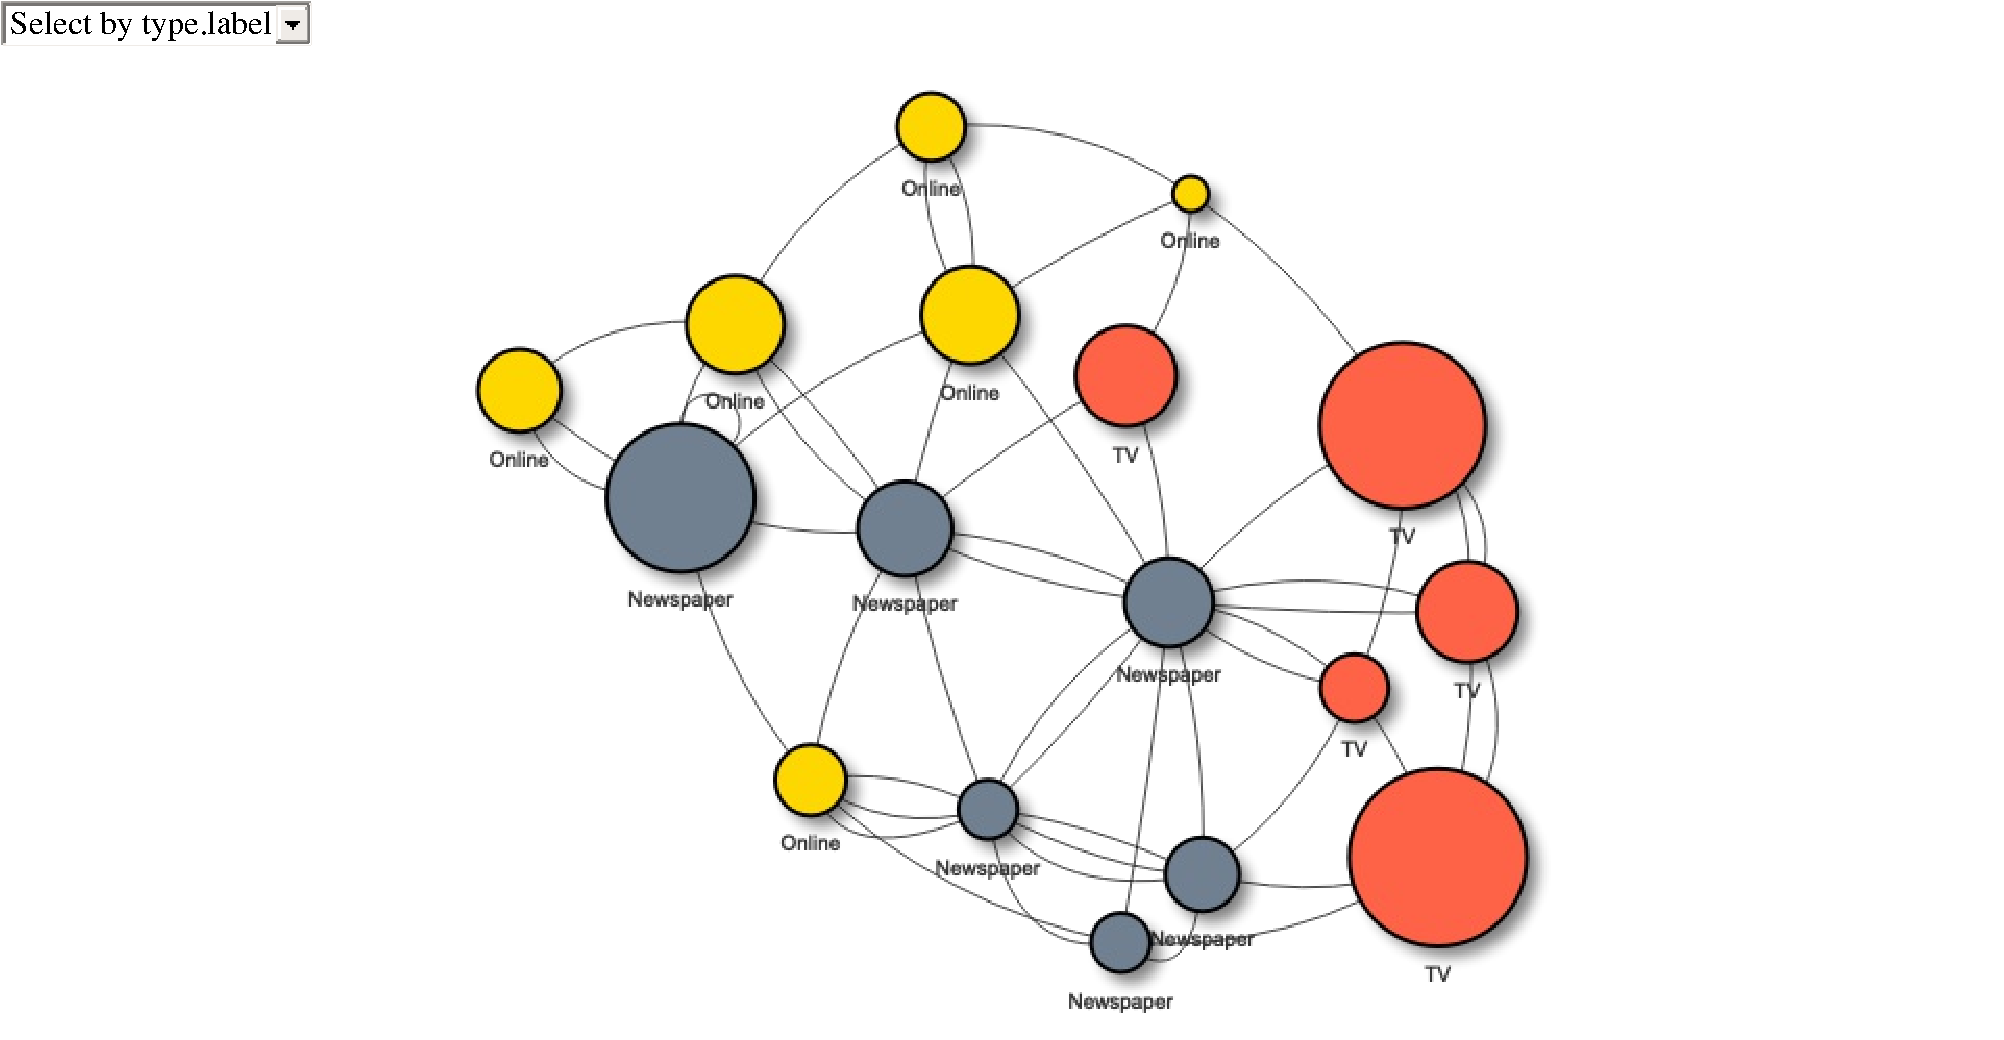
\includegraphics{R-data-viz_files/figure-latex/network-demo-1.pdf}

\section{\texorpdfstring{Maps (e.g.
\textbf{\texttt{tmap}})}{Maps (e.g. tmap)}}\label{maps-e.g.-tmap}

\begin{Shaded}
\begin{Highlighting}[]
\KeywordTok{library}\NormalTok{(tmap)}
\KeywordTok{library}\NormalTok{(tmaptools)}
\KeywordTok{suppressPackageStartupMessages}\NormalTok{(}\KeywordTok{library}\NormalTok{(sf))}

\NormalTok{london <-}\StringTok{ }\KeywordTok{st_read}\NormalTok{(}\StringTok{"demo-data/map"}\NormalTok{, }\StringTok{"London"}\NormalTok{, }\DataTypeTok{quiet =} \OtherTok{TRUE}\NormalTok{)}
\NormalTok{crime_densities <-}\StringTok{ }\KeywordTok{st_read}\NormalTok{(}\StringTok{"demo-data/map"}\NormalTok{, }\StringTok{"Crimes"}\NormalTok{, }\DataTypeTok{quiet =} \OtherTok{TRUE}\NormalTok{)}
\NormalTok{thames <-}\StringTok{ }\KeywordTok{st_read}\NormalTok{(}\StringTok{"demo-data/map"}\NormalTok{, }\StringTok{"Thames"}\NormalTok{, }\DataTypeTok{quiet =} \OtherTok{TRUE}\NormalTok{)}

\KeywordTok{tm_shape}\NormalTok{(crime_densities) }\OperatorTok{+}
\StringTok{  }\KeywordTok{tm_fill}\NormalTok{(}\DataTypeTok{col =} \StringTok{"level"}\NormalTok{, }\DataTypeTok{palette =} \StringTok{"YlOrRd"}\NormalTok{, }
    \DataTypeTok{title =} \KeywordTok{expression}\NormalTok{(}\StringTok{"Crimes per "} \OperatorTok{*}\StringTok{ }\NormalTok{km}\OperatorTok{^}\DecValTok{2}\NormalTok{)) }\OperatorTok{+}\StringTok{ }
\KeywordTok{tm_shape}\NormalTok{(london) }\OperatorTok{+}\StringTok{ }\KeywordTok{tm_borders}\NormalTok{() }\OperatorTok{+}
\KeywordTok{tm_shape}\NormalTok{(thames) }\OperatorTok{+}\StringTok{ }\KeywordTok{tm_lines}\NormalTok{(}\DataTypeTok{col =} \StringTok{"steelblue"}\NormalTok{, }\DataTypeTok{lwd =} \DecValTok{4}\NormalTok{) }\OperatorTok{+}
\KeywordTok{tm_compass}\NormalTok{(}\DataTypeTok{position =} \KeywordTok{c}\NormalTok{(}\StringTok{"left"}\NormalTok{, }\StringTok{"bottom"}\NormalTok{)) }\OperatorTok{+}
\KeywordTok{tm_scale_bar}\NormalTok{(}\DataTypeTok{position =} \KeywordTok{c}\NormalTok{(}\StringTok{"left"}\NormalTok{, }\StringTok{"bottom"}\NormalTok{)) }\OperatorTok{+}\StringTok{ }
\KeywordTok{tm_style_gray}\NormalTok{(}\DataTypeTok{title =} \StringTok{"Crimes in Greater London}\CharTok{\textbackslash{}n}\StringTok{October 2015"}\NormalTok{)}
\end{Highlighting}
\end{Shaded}

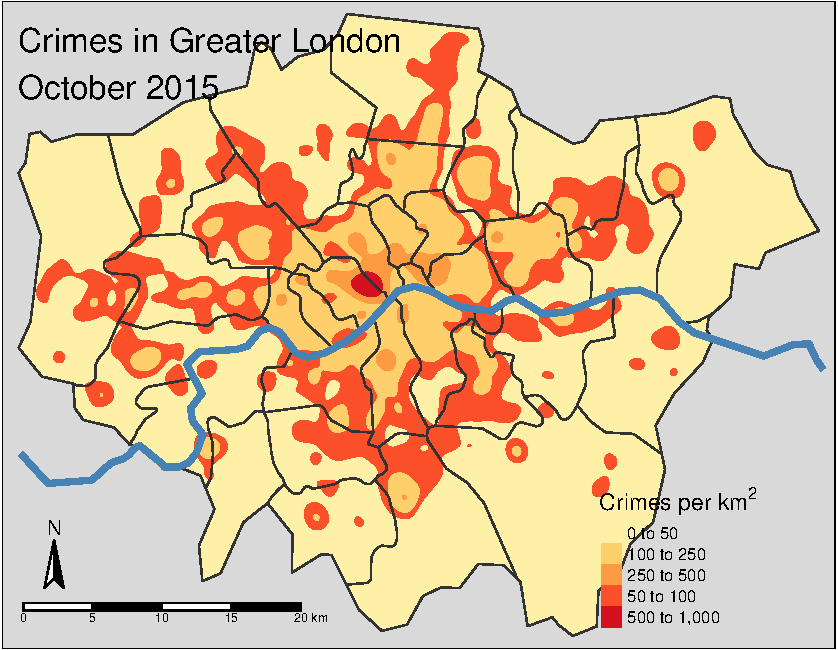
\includegraphics{R-data-viz_files/figure-latex/tmap-demo-1.pdf}

Good starting places to look for additional examples are the R Graph
Gallery: \url{https://www.r-graph-gallery.com/all-graphs/} and the CRAN
Task View: \url{https://CRAN.R-project.org/view=Graphics}.

\chapter{Interactive graphs}\label{interactive-graphs}

\begin{quote}
Learning Objectives

\begin{itemize}
\tightlist
\item
  Be aware of R interactive graphing capabilities
\item
  Understand the basic structure of a shiny app
\end{itemize}
\end{quote}

\begin{center}\rule{0.5\linewidth}{\linethickness}\end{center}

\section{plotly}\label{plotly}

\begin{Shaded}
\begin{Highlighting}[]
\KeywordTok{library}\NormalTok{(plotly)}
\end{Highlighting}
\end{Shaded}

Using the \texttt{ggplotly} function:

\begin{Shaded}
\begin{Highlighting}[]
\NormalTok{p <-}\StringTok{ }\KeywordTok{ggplot}\NormalTok{(cars, }\KeywordTok{aes}\NormalTok{(speed, dist)) }\OperatorTok{+}\StringTok{ }\KeywordTok{geom_point}\NormalTok{()}
\KeywordTok{ggplotly}\NormalTok{(p)}
\end{Highlighting}
\end{Shaded}

\includegraphics{R-data-viz_files/figure-latex/ggplotly-cars-1.pdf}

(dev. version of ggplot2 now has a \texttt{ggplotly()} function)

Using the \texttt{plot\_ly} function:

\begin{Shaded}
\begin{Highlighting}[]
\KeywordTok{library}\NormalTok{(plotly)}
\KeywordTok{plot_ly}\NormalTok{(cars, }\DataTypeTok{x =} \OperatorTok{~}\NormalTok{speed, }\DataTypeTok{y =} \OperatorTok{~}\NormalTok{dist, }\DataTypeTok{type =} \StringTok{"scatter"}\NormalTok{, }\DataTypeTok{mode =} \StringTok{"markers"}\NormalTok{)}
\end{Highlighting}
\end{Shaded}

\includegraphics{R-data-viz_files/figure-latex/plotly-cars-1.pdf}

\section{shiny}\label{shiny}

\url{https://cengel.shinyapps.io/shiny_demo/}

\begin{Shaded}
\begin{Highlighting}[]
\KeywordTok{library}\NormalTok{(shiny)}
\KeywordTok{library}\NormalTok{(ggplot2)}
\KeywordTok{inputPanel}\NormalTok{(}
    \KeywordTok{sliderInput}\NormalTok{(}\StringTok{"speed_range"}\NormalTok{, }
        \DataTypeTok{label =} \StringTok{"Range of Speed:"}\NormalTok{,}
        \DataTypeTok{min =} \KeywordTok{min}\NormalTok{(cars}\OperatorTok{$}\NormalTok{speed), }
        \DataTypeTok{max =} \KeywordTok{max}\NormalTok{(cars}\OperatorTok{$}\NormalTok{speed), }
        \DataTypeTok{value =} \KeywordTok{range}\NormalTok{(cars}\OperatorTok{$}\NormalTok{speed)))}

\KeywordTok{renderPlot}\NormalTok{(\{}
\NormalTok{    cars_sel <-}\StringTok{ }\KeywordTok{subset}\NormalTok{(cars, speed }\OperatorTok{>=}\StringTok{ }\NormalTok{input}\OperatorTok{$}\NormalTok{speed_range[}\DecValTok{1}\NormalTok{] }\OperatorTok{&}\StringTok{ }
\StringTok{                           }\NormalTok{speed }\OperatorTok{<}\StringTok{ }\NormalTok{input}\OperatorTok{$}\NormalTok{speed_range[}\DecValTok{2}\NormalTok{])}
    \KeywordTok{ggplot}\NormalTok{(cars_sel, }\KeywordTok{aes}\NormalTok{(speed, dist)) }\OperatorTok{+}\StringTok{ }\KeywordTok{geom_point}\NormalTok{()\})}
\end{Highlighting}
\end{Shaded}

For a more comprehensive example see:
\url{https://cengel.shinyapps.io/RioSlaveMarket/}

\bibliography{book.bib,packages.bib}


\end{document}
